\documentclass[journal]{IEEEtran}
\usepackage{cite}
\usepackage{amsmath,amssymb,amsfonts}
\usepackage{algorithmic}
\usepackage{graphicx}
\usepackage{textcomp}
\usepackage{xcolor}
\usepackage{booktabs}
\usepackage{url}
\usepackage{array}
\usepackage{siunitx}
% AUTO-GENERATED by Paper/generate_paper_assets.py from results/final/*.json - do not edit by hand
\newcommand{\nRaw}{572}
\newcommand{\nRawPatients}{500}
\newcommand{\nClinical}{493}
\newcommand{\nClinicalPos}{305}
\newcommand{\nMatched}{347}
\newcommand{\nMatchedPos}{237}
\newcommand{\nTrain}{277}
\newcommand{\nTest}{70}
\newcommand{\nProteinSamples}{352}
\newcommand{\nProteinRaw}{487}
\newcommand{\nProteinKept}{456}
\newcommand{\nPCAll}{129}
\newcommand{\nEvents}{9}
\newcommand{\nEventsTrain}{8}
\newcommand{\nEventsTest}{1}
\newcommand{\nEventsAll}{12}
\newcommand{\nFeatFull}{18}
\newcommand{\nFeatPreop}{13}
\newcommand{\nSites}{9}
\newcommand{\nSiteTotal}{384}
\newcommand{\nExternal}{109}
\newcommand{\bpLOC}{0.775}
\newcommand{\bpFL}{0.790}
\newcommand{\bpFR}{0.782}
\newcommand{\bpCEN}{0.789}
\newcommand{\bpBL}{0.723}
\newcommand{\bpFLminusLOC}{+0.015\ [\ensuremath{-}0.007, +0.037]}
\newcommand{\bpFRminusFL}{\ensuremath{-}0.008\ [\ensuremath{-}0.013, \ensuremath{-}0.003]}
\newcommand{\bpCENminusFL}{\ensuremath{-}0.001\ [\ensuremath{-}0.004, +0.002]}
\newcommand{\bpFLminusBL}{+0.067\ [+0.048, +0.086]}
\newcommand{\bpLcPartOne}{0.696}
\newcommand{\bpLcFrOne}{0.751}
\newcommand{\bpLcPartAll}{0.838}
\newcommand{\bpLcFrAll}{0.785}
\newcommand{\bpLooShapRho}{0.48\ [0.34, 0.62]}
\newcommand{\bpShapSizeRho}{0.51}
\newcommand{\bpMacroSites}{7.4}
\newcommand{\cvFull}{0.818}
\newcommand{\cvPreop}{0.642}
\newcommand{\cvProt}{0.574}
\newcommand{\cvFullProt}{0.659}
\newcommand{\cvSkFull}{0.824}
\newcommand{\cvRFFullProt}{0.782}
\newcommand{\cvRFFull}{0.803}
\newcommand{\cvProtDiff}{\ensuremath{-}0.159\ [\ensuremath{-}0.188, \ensuremath{-}0.130]}
\newcommand{\cvPreopDiff}{+0.176\ [+0.148, +0.203]}
\newcommand{\cvProtPreopDiff}{\ensuremath{-}0.047\ [\ensuremath{-}0.080, \ensuremath{-}0.013]}
\newcommand{\nFolds}{25}
\newcommand{\driftRedMin}{32.0}
\newcommand{\driftRedMax}{36.4}
\newcommand{\driftAvgIID}{0.206}
\newcommand{\driftAvgSkew}{0.770}
\newcommand{\driftMuZero}{0.599}
\newcommand{\driftMuOne}{0.268}
\newcommand{\sigmaTen}{5.68}
\newcommand{\sigmaFive}{10.55}
\newcommand{\sigmaTwo}{24.99}
\newcommand{\sigmaOne}{49.02}
\newcommand{\sigmaHalf}{97.01}
\newcommand{\auNoDP}{0.823}
\newcommand{\auAvgTen}{0.821}
\newcommand{\auProxTen}{0.823}
\newcommand{\auLossTen}{\ensuremath{-}0.002\ [\ensuremath{-}0.009, +0.005]}
\newcommand{\auAvgFive}{0.818}
\newcommand{\auProxFive}{0.821}
\newcommand{\auLossFive}{\ensuremath{-}0.005\ [\ensuremath{-}0.014, +0.003]}
\newcommand{\auAvgTwo}{0.800}
\newcommand{\auProxTwo}{0.812}
\newcommand{\auLossTwo}{\ensuremath{-}0.023\ [\ensuremath{-}0.038, \ensuremath{-}0.008]}
\newcommand{\auAvgOne}{0.761}
\newcommand{\auProxOne}{0.789}
\newcommand{\auLossOne}{\ensuremath{-}0.063\ [\ensuremath{-}0.087, \ensuremath{-}0.038]}
\newcommand{\auAvgHalf}{0.691}
\newcommand{\auProxHalf}{0.720}
\newcommand{\auLossHalf}{\ensuremath{-}0.132\ [\ensuremath{-}0.180, \ensuremath{-}0.085]}
\newcommand{\gridSup}{12}
\newcommand{\gridCells}{20}
\newcommand{\gridSupCtl}{3}
\newcommand{\gridNoDPmax}{0.0019}
\newcommand{\gridOneHalfMin}{0.028}
\newcommand{\gridOneHalfMax}{0.030}
\newcommand{\gridCtlOneHalfMax}{0.003}
\newcommand{\pflLocalThree}{0.754}
\newcommand{\pflProxThree}{0.811}
\newcommand{\pflPFLThree}{0.805}
\newcommand{\pflGainThree}{+0.051\ [+0.015, +0.086]}
\newcommand{\pflVsProxThree}{\ensuremath{-}0.006\ [\ensuremath{-}0.022, +0.011]}
\newcommand{\pflLocalFive}{0.796}
\newcommand{\pflProxFive}{0.817}
\newcommand{\pflPFLFive}{0.814}
\newcommand{\pflGainFive}{+0.018\ [\ensuremath{-}0.021, +0.057]}
\newcommand{\pflVsProxFive}{\ensuremath{-}0.003\ [\ensuremath{-}0.011, +0.005]}
\newcommand{\pflLocalTen}{0.785}
\newcommand{\pflProxTen}{0.841}
\newcommand{\pflPFLTen}{0.838}
\newcommand{\pflGainTen}{+0.053\ [+0.010, +0.096]}
\newcommand{\pflVsProxTen}{\ensuremath{-}0.003\ [\ensuremath{-}0.014, +0.007]}
\newcommand{\shRhoTenThree}{0.68}
\newcommand{\shRhoHalfThree}{0.25}
\newcommand{\shTSTenThree}{0.79}
\newcommand{\shTSHalfThree}{0.51}
\newcommand{\shRRHalfThree}{0.57}
\newcommand{\shLooThree}{0.68\ [0.42, 0.93]}
\newcommand{\shSizeThree}{0.55\ [0.31, 0.79]}
\newcommand{\shRThree}{5}
\newcommand{\shRhoTenFive}{0.66}
\newcommand{\shRhoHalfFive}{0.30}
\newcommand{\shTSTenFive}{0.65}
\newcommand{\shTSHalfFive}{0.41}
\newcommand{\shRRHalfFive}{0.74}
\newcommand{\shLooFive}{0.34\ [0.14, 0.54]}
\newcommand{\shSizeFive}{0.33\ [0.11, 0.55]}
\newcommand{\shRFive}{5}
\newcommand{\shRhoTenTen}{0.73}
\newcommand{\shRhoHalfTen}{0.36}
\newcommand{\shTSTenTen}{0.62}
\newcommand{\shTSHalfTen}{0.30}
\newcommand{\shRRHalfTen}{0.88}
\newcommand{\shLooTen}{0.44\ [0.30, 0.58]}
\newcommand{\shSizeTen}{0.46\ [0.35, 0.58]}
\newcommand{\shRTen}{2}
\newcommand{\miaNoDP}{0.511\ [0.489, 0.533]}
\newcommand{\miaOne}{0.510\ [0.484, 0.537]}
\newcommand{\miaHalf}{0.512\ [0.490, 0.534]}
\newcommand{\miaCtl}{0.659\ [0.640, 0.678]}
\newcommand{\miaGap}{+0.017\ [\ensuremath{-}0.007, +0.041]}
\newcommand{\shiftCovTwo}{0.765}
\newcommand{\shiftConTwo}{0.498}
\newcommand{\shiftBase}{0.826}
\newcommand{\abCen}{0.823}
\newcommand{\abAvg}{0.824}
\newcommand{\abProx}{0.826}
\newcommand{\abDPFive}{0.820}
\newcommand{\abDPOne}{0.787}
\newcommand{\abPreop}{0.659}
\newcommand{\abProt}{0.682}
\newcommand{\pNineN}{5{,}610}
\newcommand{\pNinePos}{2{,}146}
\newcommand{\pNineHosp}{19}
\newcommand{\pNineCountries}{8}
\newcommand{\pNinePrevLo}{12}
\newcommand{\pNinePrevHi}{60}
\newcommand{\pNinePrev}{38.3}
\newcommand{\pNineReps}{50}
\newcommand{\pRepNohBL}{0.827}
\newcommand{\pRepNohLOC}{0.818}
\newcommand{\pRepNohCEN}{0.827}
\newcommand{\pRepNohFL}{0.826}
\newcommand{\pRepNohFR}{0.827}
\newcommand{\pRepEttBL}{0.792}
\newcommand{\pRepEttLOC}{0.799}
\newcommand{\pRepEttCEN}{0.813}
\newcommand{\pRepEttFL}{0.803}
\newcommand{\pRepEttFR}{0.803}
\newcommand{\pSLOC}{0.829}
\newcommand{\pWLOC}{0.857}
\newcommand{\pSFL}{0.824}
\newcommand{\pWFL}{0.856}
\newcommand{\pSProx}{0.821}
\newcommand{\pWProx}{0.853}
\newcommand{\pSCEN}{0.825}
\newcommand{\pWCEN}{0.856}
\newcommand{\pSFR}{0.822}
\newcommand{\pWFR}{0.854}
\newcommand{\pSNoh}{0.834}
\newcommand{\pWNoh}{0.850}
\newcommand{\pSEtt}{0.795}
\newcommand{\pWEtt}{0.832}
\newcommand{\pDFLminusLOC}{\ensuremath{-}0.005\ [\ensuremath{-}0.015, +0.006]}
\newcommand{\pDFRminusFL}{\ensuremath{-}0.002\ [\ensuremath{-}0.002, \ensuremath{-}0.001]}
\newcommand{\pDCENminusFL}{+0.002\ [\ensuremath{-}0.001, +0.004]}
\newcommand{\pDFLminusNoh}{\ensuremath{-}0.010\ [\ensuremath{-}0.016, \ensuremath{-}0.005]}
\newcommand{\pDFLminusEtt}{+0.029\ [+0.023, +0.035]}
\newcommand{\pDProxminusFL}{\ensuremath{-}0.003\ [\ensuremath{-}0.005, \ensuremath{-}0.000]}
\newcommand{\pGainSig}{4}
\newcommand{\pLossSig}{4}
\newcommand{\pGainSizeRho}{\ensuremath{-}0.26}
\newcommand{\pLcFrOne}{0.769}
\newcommand{\pLcFrFive}{0.815}
\newcommand{\pLcFrLast}{0.830}
\newcommand{\pFrOE}{0.99}
\newcommand{\pFrSlope}{1.03}
\newcommand{\pDriftRed}{30.8}
\newcommand{\pDpLossHalf}{\ensuremath{-}0.005\ [\ensuremath{-}0.011, +0.001]}
\newcommand{\pDpLossOne}{\ensuremath{-}0.004\ [\ensuremath{-}0.008, +0.001]}
\newcommand{\pDpLossFive}{\ensuremath{-}0.002\ [\ensuremath{-}0.007, +0.003]}
\newcommand{\pProxHalfMax}{0.001}
\newcommand{\pSigmaHalf}{97}
\newcommand{\pPflSmall}{+0.039\ [+0.013, +0.065]}
\newcommand{\pPflAll}{+0.010\ [+0.005, +0.016]}
\newcommand{\pPflLarge}{+0.001\ [+0.000, +0.001]}
\newcommand{\pPflLargeLoc}{\ensuremath{-}0.005\ [\ensuremath{-}0.007, \ensuremath{-}0.004]}
\newcommand{\pNSmall}{4}
\newcommand{\pMiaNoDP}{0.500}
\newcommand{\pMiaCtl}{0.937}
\newcommand{\pLocoAvgNoh}{+0.001\ [\ensuremath{-}0.011, +0.012]}
\newcommand{\pLocoDpFive}{\ensuremath{-}0.005\ [\ensuremath{-}0.010, \ensuremath{-}0.000]}
\newcommand{\pLocoAvgCen}{\ensuremath{-}0.000\ [\ensuremath{-}0.001, +0.001]}
\newcommand{\pSlopeNoDP}{1.12\ [0.95, 1.30]}
\newcommand{\pSlopeDpFive}{0.81\ [0.70, 0.92]}
\newcommand{\pSlopeDpOne}{0.80\ [0.69, 0.91]}
\newcommand{\pSlopeNoh}{0.97\ [0.79, 1.14]}
\newcommand{\pRecalOeRaw}{0.263}
\newcommand{\pRecalOeInt}{0.071}
\newcommand{\pRecalOeDiff}{\ensuremath{-}0.193\ [\ensuremath{-}0.347, \ensuremath{-}0.038]}
\newcommand{\pRecalSlopeDpRaw}{0.81}
\newcommand{\pRecalSlopeDpLog}{0.99}
\newcommand{\pOeMin}{0.47}
\newcommand{\pOeMax}{1.30}
\newcommand{\pShRhoTen}{0.94}
\newcommand{\pShRhoHalf}{0.64}
\newcommand{\pShTSTen}{0.75}
\newcommand{\pShTSHalf}{0.40}
\newcommand{\pShRhoTwo}{0.91}
\newcommand{\pShRhoOne}{0.85}
\newcommand{\pShPhiMin}{0.029}
\newcommand{\pShPhiMax}{0.042}
\newcommand{\pShNineRhoFive}{0.90}
\newcommand{\pShNineRhoOne}{0.76}
\newcommand{\pShNineTSFive}{0.45}
\newcommand{\pShNineTSOne}{0.45}
\newcommand{\pShNineCoal}{1{,}777}
\newcommand{\pShLooRho}{0.66\ [0.56, 0.77]}
\newcommand{\pShSizeRho}{0.60}
\newcommand{\osaRhoTen}{0.90}
\newcommand{\osaRhoTwo}{0.89}
\newcommand{\osaRhoOne}{0.80}
\newcommand{\osaRhoHalf}{0.54}
\newcommand{\bmRhoTwo}{0.18}
\newcommand{\bmRhoTen}{0.47}
\newcommand{\bmRhoOne}{0.10}
\newcommand{\prRhoTen}{0.94}
\newcommand{\prRhoOne}{0.76}
\newcommand{\trueEpsOne}{33}
\newcommand{\trueEpsFive}{334}
\newcommand{\trueEpsTen}{988}
\newcommand{\osaVsBmTwo}{+0.71\ [+0.58, +0.84]}
\newcommand{\osaVsPrTwo}{\ensuremath{-}0.02\ [\ensuremath{-}0.06, +0.03]}
\newcommand{\osaVsPrOne}{+0.04\ [\ensuremath{-}0.05, +0.13]}
\newcommand{\osaNoDP}{0.96}
\newcommand{\osaSteps}{30}
\newcommand{\osaNineRhoFive}{0.95}
\newcommand{\osaNineRhoOne}{0.80}
\newcommand{\osaNineTSFive}{0.80}
\newcommand{\osaNineTSOne}{0.65}
\newcommand{\osaNineSize}{0.48}
\newcommand{\tOsaTwo}{0.39}
\newcommand{\tPrTwo}{0.52}
\newcommand{\tBmTwo}{\ensuremath{-}0.03}
\newcommand{\tOsaTen}{0.63}
\newcommand{\tPrTen}{0.72}
\newcommand{\tBmTen}{0.25}
\newcommand{\tOsaOne}{0.26}
\newcommand{\tPrOne}{0.44}
\newcommand{\tOsaNoDP}{0.91}
\newcommand{\mrRhoNoDP}{0.74}
\newcommand{\orRhoNoDP}{0.42}
\newcommand{\osaVsMrNoDP}{+0.22\ [+0.18, +0.27]}
\newcommand{\osaVsOrNoDP}{+0.54\ [+0.44, +0.65]}
\newcommand{\tMrRhoNoDP}{0.67}
\newcommand{\tOsaVsMrNoDP}{+0.24\ [+0.17, +0.31]}
\newcommand{\tHoOsaVsMrNoDP}{+0.29\ [+0.15, +0.42]}
\newcommand{\mrRhoTwo}{0.75}
\newcommand{\orRhoTwo}{0.51}
\newcommand{\osaVsMrTwo}{+0.14\ [+0.08, +0.19]}
\newcommand{\osaVsOrTwo}{+0.37\ [+0.26, +0.48]}
\newcommand{\tMrRhoTwo}{0.48}
\newcommand{\tOsaVsMrTwo}{\ensuremath{-}0.09\ [\ensuremath{-}0.27, +0.08]}
\newcommand{\tHoOsaVsMrTwo}{\ensuremath{-}0.23\ [\ensuremath{-}0.38, \ensuremath{-}0.09]}
\newcommand{\mrRhoOne}{0.65}
\newcommand{\orRhoOne}{0.50}
\newcommand{\osaVsMrOne}{+0.15\ [+0.03, +0.26]}
\newcommand{\osaVsOrOne}{+0.31\ [+0.18, +0.44]}
\newcommand{\tMrRhoOne}{0.39}
\newcommand{\tOsaVsMrOne}{\ensuremath{-}0.13\ [\ensuremath{-}0.32, +0.07]}
\newcommand{\tHoOsaVsMrOne}{\ensuremath{-}0.32\ [\ensuremath{-}0.51, \ensuremath{-}0.14]}
\newcommand{\mrRhoHalf}{0.37}
\newcommand{\orRhoHalf}{0.39}
\newcommand{\osaVsMrHalf}{+0.16\ [+0.04, +0.29]}
\newcommand{\osaVsOrHalf}{+0.14\ [+0.00, +0.28]}
\newcommand{\tMrRhoHalf}{0.26}
\newcommand{\tOsaVsMrHalf}{\ensuremath{-}0.07\ [\ensuremath{-}0.28, +0.15]}
\newcommand{\tHoOsaVsMrHalf}{\ensuremath{-}0.21\ [\ensuremath{-}0.46, +0.03]}
\newcommand{\mrRhoFive}{0.72}
\newcommand{\orRhoFive}{0.53}
\newcommand{\osaVsMrFive}{+0.18\ [+0.14, +0.22]}
\newcommand{\osaVsOrFive}{+0.37\ [+0.27, +0.47]}
\newcommand{\tMrRhoFive}{0.55}
\newcommand{\tOsaVsMrFive}{\ensuremath{-}0.03\ [\ensuremath{-}0.18, +0.12]}
\newcommand{\tHoOsaVsMrFive}{\ensuremath{-}0.12\ [\ensuremath{-}0.23, \ensuremath{-}0.00]}
\newcommand{\corrHosp}{es6}
\newcommand{\corrOsaTwo}{100\%}
\newcommand{\corrMrTwo}{70\%}
\newcommand{\corrOrTwo}{100\%}
\newcommand{\corrPrTwo}{100\%}
\newcommand{\corrBmTwo}{60\%}
\newcommand{\corrOsaOne}{95\%}
\newcommand{\corrMrOne}{80\%}
\newcommand{\corrOrOne}{100\%}
\newcommand{\corrPrOne}{100\%}
\newcommand{\corrBmOne}{45\%}
\newcommand{\corrTruth}{100\%}
\newcommand{\remOsa}{0.848}
\newcommand{\remMr}{0.849}
\newcommand{\remOr}{0.854}
\newcommand{\remTruth}{0.848}
\newcommand{\remRand}{0.853}
\newcommand{\remAll}{0.854}
\newcommand{\mlpOsaNoDP}{0.91}
\newcommand{\mlpParNoDP}{0.67}
\newcommand{\mlpMrNoDP}{0.78}
\newcommand{\mlpOsaVsMrNoDP}{+0.13\ [+0.07, +0.19]}
\newcommand{\mlpOsaTwo}{0.65}
\newcommand{\mlpParTwo}{0.65}
\newcommand{\mlpMrTwo}{0.82}
\newcommand{\mlpOsaVsMrTwo}{\ensuremath{-}0.17\ [\ensuremath{-}0.25, \ensuremath{-}0.09]}
\newcommand{\mlpOsaOne}{0.60}
\newcommand{\mlpParOne}{0.60}
\newcommand{\mlpMrOne}{0.78}
\newcommand{\mlpOsaVsMrOne}{\ensuremath{-}0.18\ [\ensuremath{-}0.29, \ensuremath{-}0.07]}
\newcommand{\mlpOsaFive}{0.68}
\newcommand{\mlpParFive}{0.52}
\newcommand{\mlpMrFive}{0.82}
\newcommand{\mlpOsaVsMrFive}{\ensuremath{-}0.14\ [\ensuremath{-}0.19, \ensuremath{-}0.09]}
\newcommand{\mlpOsaHalf}{0.42}
\newcommand{\mlpParHalf}{0.44}
\newcommand{\mlpMrHalf}{0.74}
\newcommand{\mlpOsaVsMrHalf}{\ensuremath{-}0.32\ [\ensuremath{-}0.46, \ensuremath{-}0.18]}
\newcommand{\mlpBmTwo}{0.16}
\newcommand{\mlpOsaVsBmTwo}{+0.47\ [\ensuremath{-}0.34, +1.28]}
\newcommand{\mlpTrueEpsTwo}{85}
\newcommand{\mlpBmOne}{0.05}
\newcommand{\mlpOsaVsBmOne}{+0.46\ [\ensuremath{-}0.42, +1.35]}
\newcommand{\mlpTrueEpsOne}{33}
\newcommand{\mlpBmSeeds}{5}
\newcommand{\blAvg}{0.816}
\newcommand{\blAvgLong}{0.818}
\newcommand{\blAdam}{0.818}
\newcommand{\blScaf}{0.816}
\newcommand{\blMLP}{0.821}
\newcommand{\blGB}{0.824}
\newcommand{\blRF}{0.820}
\newcommand{\blCMLP}{0.828}
\newcommand{\blCLR}{0.819}
\newcommand{\blDLong}{+0.002\ [+0.001, +0.003]}
\newcommand{\blDAdam}{+0.002\ [+0.000, +0.005]}
\newcommand{\blDMLP}{+0.005\ [+0.001, +0.009]}
\newcommand{\blDGB}{+0.009\ [+0.004, +0.014]}
\newcommand{\blDScaf}{\ensuremath{-}0.000\ [\ensuremath{-}0.001, +0.000]}
\newcommand{\blLMLP}{+0.005\ [\ensuremath{-}0.000, +0.010]}
\newcommand{\blLGB}{\ensuremath{-}0.003\ [\ensuremath{-}0.011, +0.004]}
\newcommand{\blScafDrift}{65}
\newcommand{\blProxDrift}{31}
\newcommand{\blDpScaf}{+0.000\ [\ensuremath{-}0.000, +0.000]}
\newcommand{\blDpAdam}{\ensuremath{-}0.004\ [\ensuremath{-}0.008, +0.000]}
\newcommand{\blDpProx}{\ensuremath{-}0.001\ [\ensuremath{-}0.004, +0.001]}
\newcommand{\btScafLow}{\ensuremath{-}0.004\ [\ensuremath{-}0.007, \ensuremath{-}0.001]}
\newcommand{\btAdamLow}{\ensuremath{-}0.016\ [\ensuremath{-}0.033, +0.001]}
\newcommand{\btMLPLow}{\ensuremath{-}0.013\ [\ensuremath{-}0.028, +0.001]}
\newcommand{\btAvgLow}{0.827}
\newcommand{\btScafMid}{+0.000\ [\ensuremath{-}0.002, +0.003]}
\newcommand{\btAdamMid}{\ensuremath{-}0.012\ [\ensuremath{-}0.025, +0.002]}
\newcommand{\btMLPMid}{\ensuremath{-}0.017\ [\ensuremath{-}0.030, \ensuremath{-}0.004]}
\newcommand{\btAvgMid}{0.822}
\newcommand{\btGB}{0.786}
\newcommand{\btCLR}{0.825}
\newcommand{\cvgFLminusLOC}{\ensuremath{-}0.005\ [\ensuremath{-}0.016, +0.006]}
\newcommand{\cvgFLminusNoh}{\ensuremath{-}0.008\ [\ensuremath{-}0.013, \ensuremath{-}0.003]}
\newcommand{\cvgFRminusFL}{\ensuremath{-}0.001\ [\ensuremath{-}0.001, \ensuremath{-}0.001]}
\newcommand{\cvgCENminusFL}{+0.001\ [\ensuremath{-}0.000, +0.003]}
\newcommand{\cvgFL}{0.826}
\newcommand{\cvgWFL}{0.858}
\newcommand{\cvgWNoh}{0.850}
\newcommand{\ssSigFull}{49.0}
\newcommand{\ssSigThree}{25.6}
\newcommand{\ssSigOne}{15.6}
\newcommand{\ssTThreeOne}{\ensuremath{-}0.009\ [\ensuremath{-}0.042, +0.025]}
\newcommand{\ssTThreeHalf}{\ensuremath{-}0.010\ [\ensuremath{-}0.070, +0.051]}
\newcommand{\ssTOneOne}{\ensuremath{-}0.009\ [\ensuremath{-}0.025, +0.008]}
\newcommand{\ssPThreeOne}{+0.001\ [\ensuremath{-}0.003, +0.004]}
\newcommand{\ssTFullOne}{0.761}
\newcommand{\ssTThreeOneAbs}{0.752}
\newcommand{\pxLSizeNoDP}{0.08}
\newcommand{\pxdLSizeNoDP}{+0.88\ [+0.79, +0.97]}
\newcommand{\pxLPosNoDP}{0.02}
\newcommand{\pxdLPosNoDP}{+0.94\ [+0.85, +1.03]}
\newcommand{\pxLStatNoDP}{\ensuremath{-}0.18}
\newcommand{\pxdLStatNoDP}{+1.14\ [+1.06, +1.21]}
\newcommand{\pxLOwnNoDP}{0.36}
\newcommand{\pxdLOwnNoDP}{+0.60\ [+0.44, +0.76]}
\newcommand{\pxLRefNoDP}{0.93}
\newcommand{\pxdLRefNoDP}{+0.03\ [+0.01, +0.05]}
\newcommand{\pxLLooNoDP}{0.85}
\newcommand{\pxdLLooNoDP}{+0.12\ [+0.08, +0.15]}
\newcommand{\pxLOsaNoDP}{0.96}
\newcommand{\pxLMrNoDP}{0.74}
\newcommand{\pxdLMrNoDP}{+0.22\ [+0.18, +0.27]}
\newcommand{\pxLOrNoDP}{0.42}
\newcommand{\pxdLOrNoDP}{+0.54\ [+0.44, +0.65]}
\newcommand{\pxLSizeFive}{0.08}
\newcommand{\pxdLSizeFive}{+0.82\ [+0.72, +0.92]}
\newcommand{\pxLPosFive}{0.02}
\newcommand{\pxdLPosFive}{+0.88\ [+0.78, +0.99]}
\newcommand{\pxLStatFive}{\ensuremath{-}0.18}
\newcommand{\pxdLStatFive}{+1.08\ [+1.00, +1.16]}
\newcommand{\pxLOwnFive}{0.26}
\newcommand{\pxdLOwnFive}{+0.64\ [+0.48, +0.80]}
\newcommand{\pxLRefFive}{0.88}
\newcommand{\pxdLRefFive}{+0.02\ [\ensuremath{-}0.01, +0.05]}
\newcommand{\pxLLooFive}{0.79}
\newcommand{\pxdLLooFive}{+0.12\ [+0.08, +0.15]}
\newcommand{\pxLOsaFive}{0.90}
\newcommand{\pxLMrFive}{0.72}
\newcommand{\pxdLMrFive}{+0.18\ [+0.14, +0.22]}
\newcommand{\pxLOrFive}{0.53}
\newcommand{\pxdLOrFive}{+0.37\ [+0.27, +0.47]}
\newcommand{\pxLSizeTwo}{0.08}
\newcommand{\pxdLSizeTwo}{+0.80\ [+0.70, +0.91]}
\newcommand{\pxLPosTwo}{0.02}
\newcommand{\pxdLPosTwo}{+0.87\ [+0.76, +0.97]}
\newcommand{\pxLStatTwo}{\ensuremath{-}0.18}
\newcommand{\pxdLStatTwo}{+1.06\ [+0.98, +1.15]}
\newcommand{\pxLOwnTwo}{0.25}
\newcommand{\pxdLOwnTwo}{+0.64\ [+0.49, +0.79]}
\newcommand{\pxLRefTwo}{0.85}
\newcommand{\pxdLRefTwo}{+0.04\ [\ensuremath{-}0.00, +0.08]}
\newcommand{\pxLLooTwo}{0.77}
\newcommand{\pxdLLooTwo}{+0.11\ [+0.08, +0.15]}
\newcommand{\pxLOsaTwo}{0.89}
\newcommand{\pxLMrTwo}{0.75}
\newcommand{\pxdLMrTwo}{+0.14\ [+0.08, +0.19]}
\newcommand{\pxLOrTwo}{0.51}
\newcommand{\pxdLOrTwo}{+0.37\ [+0.26, +0.48]}
\newcommand{\pxLSizeOne}{0.08}
\newcommand{\pxdLSizeOne}{+0.72\ [+0.61, +0.83]}
\newcommand{\pxLPosOne}{0.02}
\newcommand{\pxdLPosOne}{+0.78\ [+0.67, +0.90]}
\newcommand{\pxLStatOne}{\ensuremath{-}0.18}
\newcommand{\pxdLStatOne}{+0.98\ [+0.88, +1.08]}
\newcommand{\pxLOwnOne}{0.26}
\newcommand{\pxdLOwnOne}{+0.54\ [+0.42, +0.66]}
\newcommand{\pxLRefOne}{0.71}
\newcommand{\pxdLRefOne}{+0.10\ [+0.05, +0.14]}
\newcommand{\pxLLooOne}{0.74}
\newcommand{\pxdLLooOne}{+0.06\ [+0.01, +0.11]}
\newcommand{\pxLOsaOne}{0.80}
\newcommand{\pxLMrOne}{0.65}
\newcommand{\pxdLMrOne}{+0.15\ [+0.03, +0.26]}
\newcommand{\pxLOrOne}{0.50}
\newcommand{\pxdLOrOne}{+0.31\ [+0.18, +0.44]}
\newcommand{\pxSSizeNoDP}{0.74}
\newcommand{\pxdSSizeNoDP}{+0.21\ [+0.19, +0.24]}
\newcommand{\pxSPosNoDP}{0.50}
\newcommand{\pxdSPosNoDP}{+0.46\ [+0.43, +0.49]}
\newcommand{\pxSStatNoDP}{0.72}
\newcommand{\pxdSStatNoDP}{+0.23\ [+0.17, +0.29]}
\newcommand{\pxSOwnNoDP}{0.40}
\newcommand{\pxdSOwnNoDP}{+0.55\ [+0.45, +0.65]}
\newcommand{\pxSRefNoDP}{0.94}
\newcommand{\pxdSRefNoDP}{+0.01\ [\ensuremath{-}0.02, +0.03]}
\newcommand{\pxSLooNoDP}{0.59}
\newcommand{\pxdSLooNoDP}{+0.37\ [+0.28, +0.45]}
\newcommand{\pxSOsaNoDP}{0.95}
\newcommand{\pxSMrNoDP}{0.86}
\newcommand{\pxdSMrNoDP}{+0.10\ [+0.05, +0.14]}
\newcommand{\pxSOrNoDP}{0.79}
\newcommand{\pxdSOrNoDP}{+0.16\ [+0.12, +0.21]}
\newcommand{\pxSSizeFive}{0.74}
\newcommand{\pxdSSizeFive}{+0.11\ [+0.07, +0.16]}
\newcommand{\pxSPosFive}{0.50}
\newcommand{\pxdSPosFive}{+0.36\ [+0.31, +0.40]}
\newcommand{\pxSStatFive}{0.72}
\newcommand{\pxdSStatFive}{+0.13\ [+0.07, +0.19]}
\newcommand{\pxSOwnFive}{0.49}
\newcommand{\pxdSOwnFive}{+0.37\ [+0.23, +0.50]}
\newcommand{\pxSRefFive}{0.85}
\newcommand{\pxdSRefFive}{+0.00\ [\ensuremath{-}0.02, +0.02]}
\newcommand{\pxSLooFive}{0.36}
\newcommand{\pxdSLooFive}{+0.49\ [+0.40, +0.58]}
\newcommand{\pxSOsaFive}{0.85}
\newcommand{\pxSMrFive}{0.83}
\newcommand{\pxdSMrFive}{+0.03\ [\ensuremath{-}0.00, +0.06]}
\newcommand{\pxSOrFive}{0.81}
\newcommand{\pxdSOrFive}{+0.04\ [\ensuremath{-}0.00, +0.08]}
\newcommand{\pxSBmFive}{0.68}
\newcommand{\pxdSBmFive}{+0.17\ [+0.09, +0.25]}
\newcommand{\pxSSizeTwo}{0.74}
\newcommand{\pxdSSizeTwo}{+0.05\ [\ensuremath{-}0.01, +0.10]}
\newcommand{\pxSPosTwo}{0.50}
\newcommand{\pxdSPosTwo}{+0.29\ [+0.24, +0.35]}
\newcommand{\pxSStatTwo}{0.72}
\newcommand{\pxdSStatTwo}{+0.06\ [\ensuremath{-}0.01, +0.14]}
\newcommand{\pxSOwnTwo}{0.54}
\newcommand{\pxdSOwnTwo}{+0.24\ [+0.12, +0.36]}
\newcommand{\pxSRefTwo}{0.79}
\newcommand{\pxdSRefTwo}{\ensuremath{-}0.00\ [\ensuremath{-}0.06, +0.06]}
\newcommand{\pxSLooTwo}{0.34}
\newcommand{\pxdSLooTwo}{+0.44\ [+0.34, +0.54]}
\newcommand{\pxSOsaTwo}{0.79}
\newcommand{\pxSMrTwo}{0.78}
\newcommand{\pxdSMrTwo}{+0.00\ [\ensuremath{-}0.06, +0.06]}
\newcommand{\pxSOrTwo}{0.74}
\newcommand{\pxdSOrTwo}{+0.05\ [\ensuremath{-}0.03, +0.13]}
\newcommand{\pxSBmTwo}{0.45}
\newcommand{\pxdSBmTwo}{+0.34\ [+0.24, +0.44]}
\newcommand{\pxSSizeOne}{0.74}
\newcommand{\pxdSSizeOne}{\ensuremath{-}0.06\ [\ensuremath{-}0.15, +0.02]}
\newcommand{\pxSPosOne}{0.50}
\newcommand{\pxdSPosOne}{+0.18\ [+0.10, +0.27]}
\newcommand{\pxSStatOne}{0.72}
\newcommand{\pxdSStatOne}{\ensuremath{-}0.04\ [\ensuremath{-}0.15, +0.06]}
\newcommand{\pxSOwnOne}{0.56}
\newcommand{\pxdSOwnOne}{+0.12\ [\ensuremath{-}0.00, +0.24]}
\newcommand{\pxSRefOne}{0.72}
\newcommand{\pxdSRefOne}{\ensuremath{-}0.04\ [\ensuremath{-}0.10, +0.02]}
\newcommand{\pxSLooOne}{0.34}
\newcommand{\pxdSLooOne}{+0.34\ [+0.25, +0.44]}
\newcommand{\pxSOsaOne}{0.68}
\newcommand{\pxSMrOne}{0.74}
\newcommand{\pxdSMrOne}{\ensuremath{-}0.06\ [\ensuremath{-}0.15, +0.03]}
\newcommand{\pxSOrOne}{0.59}
\newcommand{\pxdSOrOne}{+0.09\ [\ensuremath{-}0.01, +0.19]}
\newcommand{\pxSBmOne}{0.29}
\newcommand{\pxdSBmOne}{+0.39\ [+0.25, +0.52]}
\newcommand{\pxCSizeNoDP}{0\%}
\newcommand{\pxCStatNoDP}{0\%}
\newcommand{\pxCOwnNoDP}{95\%}
\newcommand{\pxCRefNoDP}{100\%}
\newcommand{\pxCLooNoDP}{0\%}
\newcommand{\pxCOsaNoDP}{100\%}
\newcommand{\pxCSizeTwo}{0\%}
\newcommand{\pxCStatTwo}{0\%}
\newcommand{\pxCOwnTwo}{100\%}
\newcommand{\pxCRefTwo}{100\%}
\newcommand{\pxCLooTwo}{0\%}
\newcommand{\pxCOsaTwo}{100\%}
\newcommand{\pxCSizeOne}{0\%}
\newcommand{\pxCStatOne}{0\%}
\newcommand{\pxCOwnOne}{90\%}
\newcommand{\pxCRefOne}{100\%}
\newcommand{\pxCLooOne}{0\%}
\newcommand{\pxCOsaOne}{95\%}
\newcommand{\pxSmallMin}{16}
\newcommand{\pxSmallMax}{266}
\newcommand{\pxSmallHosp}{nl, it, es4, es5, de2, gb, es1, es8, es3, es2}
\newcommand{\accMcNineteenOne}{52}
\newcommand{\accMcTenOne}{34}
\newcommand{\accMcFiftyOne}{103}
\newcommand{\accFourOne}{2.9}
\newcommand{\accFourTwo}{6.1}
\newcommand{\hrSizeNoDP}{\ensuremath{-}0.38}
\newcommand{\hrdSizeNoDP}{+1.30\ [+1.12, +1.48]}
\newcommand{\hrStatNoDP}{\ensuremath{-}0.38}
\newcommand{\hrdStatNoDP}{+1.30\ [+1.12, +1.48]}
\newcommand{\hrOwnNoDP}{\ensuremath{-}0.18}
\newcommand{\hrdOwnNoDP}{+1.10\ [+0.84, +1.36]}
\newcommand{\hrRefNoDP}{0.76}
\newcommand{\hrdRefNoDP}{+0.16\ [\ensuremath{-}0.01, +0.33]}
\newcommand{\hrLooNoDP}{0.82}
\newcommand{\hrdLooNoDP}{+0.10\ [\ensuremath{-}0.00, +0.20]}
\newcommand{\hrOsaNoDP}{0.92}
\newcommand{\hrMrNoDP}{0.70}
\newcommand{\hrdMrNoDP}{+0.22\ [+0.05, +0.39]}
\newcommand{\hrOrNoDP}{0.23}
\newcommand{\hrdOrNoDP}{+0.69\ [+0.46, +0.92]}
\newcommand{\hrSizeFive}{\ensuremath{-}0.38}
\newcommand{\hrdSizeFive}{+0.89\ [+0.51, +1.27]}
\newcommand{\hrStatFive}{\ensuremath{-}0.38}
\newcommand{\hrdStatFive}{+0.89\ [+0.51, +1.27]}
\newcommand{\hrOwnFive}{\ensuremath{-}0.17}
\newcommand{\hrdOwnFive}{+0.68\ [+0.28, +1.08]}
\newcommand{\hrRefFive}{0.42}
\newcommand{\hrdRefFive}{+0.09\ [\ensuremath{-}0.05, +0.23]}
\newcommand{\hrLooFive}{0.69}
\newcommand{\hrdLooFive}{\ensuremath{-}0.18\ [\ensuremath{-}0.39, +0.03]}
\newcommand{\hrOsaFive}{0.51}
\newcommand{\hrMrFive}{0.64}
\newcommand{\hrdMrFive}{\ensuremath{-}0.13\ [\ensuremath{-}0.38, +0.12]}
\newcommand{\hrOrFive}{0.29}
\newcommand{\hrdOrFive}{+0.22\ [+0.01, +0.43]}
\newcommand{\hrBmFive}{\ensuremath{-}0.02}
\newcommand{\hrdBmFive}{+0.53\ [+0.17, +0.89]}
\newcommand{\hrPrFive}{0.34}
\newcommand{\hrdPrFive}{+0.17\ [\ensuremath{-}0.18, +0.52]}
\newcommand{\hrSizeTwo}{\ensuremath{-}0.38}
\newcommand{\hrdSizeTwo}{+0.53\ [+0.28, +0.78]}
\newcommand{\hrStatTwo}{\ensuremath{-}0.38}
\newcommand{\hrdStatTwo}{+0.53\ [+0.28, +0.78]}
\newcommand{\hrOwnTwo}{\ensuremath{-}0.31}
\newcommand{\hrdOwnTwo}{+0.46\ [+0.19, +0.73]}
\newcommand{\hrRefTwo}{\ensuremath{-}0.04}
\newcommand{\hrdRefTwo}{+0.19\ [+0.05, +0.33]}
\newcommand{\hrLooTwo}{0.42}
\newcommand{\hrdLooTwo}{\ensuremath{-}0.27\ [\ensuremath{-}0.59, +0.05]}
\newcommand{\hrOsaTwo}{0.15}
\newcommand{\hrMrTwo}{0.45}
\newcommand{\hrdMrTwo}{\ensuremath{-}0.30\ [\ensuremath{-}0.59, \ensuremath{-}0.01]}
\newcommand{\hrOrTwo}{0.18}
\newcommand{\hrdOrTwo}{\ensuremath{-}0.03\ [\ensuremath{-}0.34, +0.28]}
\newcommand{\hrBmTwo}{\ensuremath{-}0.18}
\newcommand{\hrdBmTwo}{+0.33\ [+0.05, +0.61]}
\newcommand{\hrPrTwo}{\ensuremath{-}0.09}
\newcommand{\hrdPrTwo}{+0.24\ [\ensuremath{-}0.04, +0.52]}
\newcommand{\hrSizeOne}{\ensuremath{-}0.38}
\newcommand{\hrdSizeOne}{+0.20\ [+0.02, +0.38]}
\newcommand{\hrStatOne}{\ensuremath{-}0.38}
\newcommand{\hrdStatOne}{+0.20\ [+0.02, +0.38]}
\newcommand{\hrOwnOne}{\ensuremath{-}0.30}
\newcommand{\hrdOwnOne}{+0.12\ [\ensuremath{-}0.16, +0.40]}
\newcommand{\hrRefOne}{\ensuremath{-}0.34}
\newcommand{\hrdRefOne}{+0.16\ [\ensuremath{-}0.01, +0.33]}
\newcommand{\hrLooOne}{0.18}
\newcommand{\hrdLooOne}{\ensuremath{-}0.36\ [\ensuremath{-}0.68, \ensuremath{-}0.04]}
\newcommand{\hrOsaOne}{\ensuremath{-}0.18}
\newcommand{\hrMrOne}{\ensuremath{-}0.35}
\newcommand{\hrdMrOne}{+0.17\ [\ensuremath{-}0.05, +0.39]}
\newcommand{\hrOrOne}{0.04}
\newcommand{\hrdOrOne}{\ensuremath{-}0.22\ [\ensuremath{-}0.59, +0.15]}
\newcommand{\hrBmOne}{\ensuremath{-}0.15}
\newcommand{\hrdBmOne}{\ensuremath{-}0.03\ [\ensuremath{-}0.32, +0.26]}
\newcommand{\hrPrOne}{\ensuremath{-}0.27}
\newcommand{\hrdPrOne}{+0.09\ [\ensuremath{-}0.12, +0.30]}
\newcommand{\hrCOsaTwo}{100\%}
\newcommand{\hrCRefTwo}{100\%}
\newcommand{\hrCSizeTwo}{0\%}
\newcommand{\hrCOsaOne}{80\%}
\newcommand{\hrCRefOne}{85\%}
\newcommand{\hrCSizeOne}{0\%}
\newcommand{\hrN}{920}
\newcommand{\hrFeat}{20}
\newcommand{\hrAuc}{0.85}
\newcommand{\hrCorrupt}{Budapest}
\newcommand{\hrPhiMin}{0.085}
\newcommand{\hrPhiMax}{0.101}
\newcommand{\hrTrueOne}{2.9}
\newcommand{\hrTrueTwo}{6.1}
\newcommand{\nuLarge}{114}
\newcommand{\nuSmall}{45}
\newcommand{\nuHeart}{43}
\newcommand{\nuMlp}{26}
\newcommand{\nsCrossTwo}{21}
\newcommand{\nsCrossOneMax}{38}
\newcommand{\nsCrossOneMin}{26}
\newcommand{\nsSpear}{0.57}
\newcommand{\nsLowerCount}{5}
\newcommand{\nsAFortyFiveNu}{45}
\newcommand{\nsAFortyFiveTwo}{+0.18\ [+0.08, +0.29]}
\newcommand{\nsAFortyFiveOne}{+0.12\ [\ensuremath{-}0.04, +0.27]}
\newcommand{\nsATwentyEightNu}{28}
\newcommand{\nsATwentyEightTwo}{+0.12\ [+0.00, +0.24]}
\newcommand{\nsATwentyEightOne}{+0.04\ [\ensuremath{-}0.07, +0.16]}
\newcommand{\nsASeventeenNu}{17}
\newcommand{\nsASeventeenTwo}{\ensuremath{-}0.09\ [\ensuremath{-}0.20, +0.03]}
\newcommand{\nsASeventeenOne}{\ensuremath{-}0.18\ [\ensuremath{-}0.32, \ensuremath{-}0.03]}
\newcommand{\nsASixtyEightNu}{68}
\newcommand{\nsASixtyEightTwo}{+0.08\ [+0.00, +0.16]}
\newcommand{\nsASixtyEightOne}{+0.14\ [+0.02, +0.26]}
\newcommand{\nsBTwentyOneNu}{57}
\newcommand{\nsBTwentyOneTwo}{+0.07\ [\ensuremath{-}0.03, +0.18]}
\newcommand{\nsBTwentyOneOne}{+0.13\ [+0.01, +0.24]}
\newcommand{\nsBFiftyNu}{40}
\newcommand{\nsBFiftyTwo}{+0.05\ [\ensuremath{-}0.02, +0.12]}
\newcommand{\nsBFiftyOne}{+0.01\ [\ensuremath{-}0.08, +0.10]}
\newcommand{\nsBHundredNu}{29}
\newcommand{\nsBHundredTwo}{+0.05\ [\ensuremath{-}0.02, +0.11]}
\newcommand{\nsBHundredOne}{\ensuremath{-}0.07\ [\ensuremath{-}0.15, +0.00]}


\begin{document}

\title{Privacy, Heterogeneity and Contribution Valuation in Federated Prostate Cancer Risk Prediction: Evidence from 19 Real Hospitals and TCGA-PRAD}

\author{Ponnaluri~Jeyanth,
        Pudota~Jaideep,
        and~M.~V.~P.~Chandra~Sekhara~Rao%
\thanks{P. Jeyanth and P. Jaideep are with the Department of Computer Science and Engineering (Data Science), R.V.R. \& J.C. College of Engineering, Guntur, India (e-mail: jeyanthponnaluri08@gmail.com; pudotajaideep@gmail.com).}%
\thanks{M. V. P. Chandra Sekhara Rao is Professor and Head of the Department of Computer Science and Engineering (Data Science), R.V.R. \& J.C. College of Engineering, Guntur, India (e-mail: manukondach@gmail.com).}%
\thanks{Code, data provenance and all results: \protect\url{https://github.com/JeyanthPonnaluri/Mini_Project_RVR}.}}

\markboth{Manuscript submitted to IEEE Journal of Biomedical and Health Informatics}%
{Jeyanth \MakeLowercase{\textit{et al.}}: Privacy, Heterogeneity and Contribution Valuation in Federated Prostate Cancer Risk Prediction}

\maketitle

\begin{abstract}
Federated learning lets hospitals train a shared model without exchanging patient records, but its value depends on how privacy constraints, statistical heterogeneity and incentives interact. We study these interactions with one leakage-free, validated pipeline and 20 paired splits per experiment. The primary cohort is the exact 19-hospital, \pNineN{}-patient pre-biopsy collection of a recent hospital-participation study (PCa-19: clinically significant cancer from age, PSA, prostate volume and PI-RADS); the secondary cohort is post-surgical staging on TCGA-PRAD. Our re-implementation reproduces the base paper's protocol number for number, and its sustainability finding holds under ours: joining a federation gives no significant average local gain, free-riders obtain nearly the same model, and federated training matches pooled training. Leave-one-country-out validation shows that discrimination transports across countries but calibration does not; differential privacy (DP) costs little AUC but makes predictions over-confident (calibration slope $\pSlopeDpFive$ at $\varepsilon=5$), and local recalibration on 20\% of a new country's patients repairs both. SCAFFOLD, FedAdam, a federated MLP and centralised gradient boosting do not improve on federated logistic regression, and Poisson-subsampled DP with sampled-Gaussian accounting does not improve utility over full-batch DP. We then show that the standard way of valuing hospitals under DP, retraining every coalition with DP, silently spends the budget hundreds of times over (a per-run $\varepsilon=1$ costs $\varepsilon\approx\trueEpsOne$ for ten hospitals), and at an honest budget it loses the contribution ranking ($\rho=\bmRhoOne$ at $\varepsilon=1$). We propose OSA-Shapley, which values all coalitions by post-processing one DP-trained model per hospital. At the same privacy cost it recovers the exact Shapley ranking far better ($\rho=\osaRhoTwo$ at $\varepsilon=2$ and \osaRhoOne{} at $\varepsilon=1$), matches costly retraining, and makes exact valuation of all 19 hospitals tractable. All numbers are regenerated from code and checked by 34 automated tests.
\end{abstract}

\begin{IEEEkeywords}
Federated Learning, Differential Privacy, FedProx, Non-IID Learning, Prostate Cancer, Data Valuation, Shapley Value, Membership Inference.
\end{IEEEkeywords}

\section{Introduction}
\IEEEPARstart{R}{isk} prediction for prostate cancer guides two key decisions: whether a man with raised PSA needs a biopsy, and, after surgery, how advanced the tumour is. Both are central to clinical risk stratification and treatment planning. Accurate identification of disease severity determines whether a patient undergoes radical prostatectomy, radiotherapy, active surveillance, or systemic androgen deprivation therapy. Machine learning models trained on combined clinical and molecular profiles can support clinicians in identifying high-risk disease. However, clinical and genomic cohorts are frequently isolated across institutions. Centralizing these datasets into a single repository is often impossible due to institutional barriers and data protection regulations (e.g., HIPAA and GDPR).

Federated Learning (FL) has emerged as a promising collaborative paradigm to address these limitations. Under FL, clinical sites cooperatively train a global model by sharing local update gradients or parameters rather than raw clinical records. Yet, clinical federated networks face three major challenges. First, statistical heterogeneity (non-IID data distributions) arising from variations in clinical protocols, regional demographics, and equipment calibration causes client update parameters to diverge from the global optimization trajectory, leading to client drift and suboptimal convergence. Second, the transfer of gradient updates is vulnerable to privacy reconstruction and membership leakage, requiring formal privacy guarantees such as Differential Privacy (DP). Third, participant sites require reliable contribution valuation mechanisms to justify collaboration, but naive metrics fail to capture marginal contributions.

Prior research has largely examined these challenges in isolation. The interactions between statistical heterogeneity, differential privacy noise, local personalization, and contribution valuation remain poorly understood. For example, adding differential privacy noise to local updates disrupts optimization paths, and the severity of this disruption depends on the non-IID label skew across hospitals. Similarly, privacy noise alters computed game-theoretic contribution scores, potentially destabilizing incentive allocation.

To address these gaps, we systematically study the central research question: **How do privacy constraints and statistical heterogeneity jointly affect federated clinical model utility, local adaptation, and participant contribution valuation?** We construct a multi-dimensional conceptual model to characterize these relationships: clinical heterogeneity leads to client optimization drift, which is stabilized by FedProx regularization; this interaction occurs alongside privacy perturbation under sample-level differential privacy, establishing a privacy--utility trade-off; these combined constraints affect both global model utility and local personalized adaptation, which ultimately alters participant contribution valuation and its associated economic incentive allocation. The conceptual framework tracking these causal interactions is depicted in Fig. \ref{fig:conceptual_map}.

We characterise these interactions on two cohorts. The primary cohort is the base paper's own 19-hospital pre-biopsy collection (PCa-19, \pNineN{} men, \pNineCountries{} countries), released by Kazlouski \emph{et al.}\ \cite{Kazlouski2025HospitalParticipation}. It provides real hospitals, PSA and MRI, and enough countries for external validation. The secondary cohort is TCGA-PRAD, a small post-surgical staging cohort on which privacy is expensive. Our main contributions are:
\begin{itemize}
    \item \textbf{OSA-Shapley, privacy-honest valuation}: we show that valuing hospitals by retraining coalitions under DP spends the privacy budget $2^{K-1}$ times, and propose a valuation that post-processes one DP-trained model per hospital. At equal privacy it recovers the exact Shapley ranking far better than retraining (Spearman $\rho$ at $\varepsilon=2$: \osaRhoTwo{} vs \bmRhoTwo{}) and allows exact valuation of 19 hospitals.
    \item \textbf{Stronger baselines and accounting}: SCAFFOLD, FedAdam, federated and centralised non-linear models, a converged FedAvg, and Poisson-subsampled DP with sampled-Gaussian accounting; none changes the conclusions.
    \item \textbf{Exact reproduction}: our re-implementation of the authors' public protocol gives the same numbers as their code; under our protocol the sustainability finding holds (FL$-$LOC $=\pDFLminusLOC$, FR$-$FL $=\pDFRminusFL$), but a published single-country calculator is not beaten on hospital-averaged AUC.
    \item \textbf{External validation and calibration}: in leave-one-country-out validation, federated models match pooled training and the published calculator in discrimination, but calibration varies by country, and DP makes predictions over-confident (slope $\pSlopeDpFive$ at $\varepsilon=5$); local recalibration on 20\% of a new country's patients repairs both.
    \item \textbf{Privacy is nearly free at scale}: with \pNineN{} patients the AUC loss at $\varepsilon=0.5$ is $\pDpLossHalf$, against $\auLossOne$ at $\varepsilon=1$ on TCGA.
    \item \textbf{Valuation under privacy}: Shapley rankings of real hospitals hold at weak privacy (Spearman \pShRhoTen{} at $\varepsilon=10$) but break down at strong privacy (\pShRhoHalf{} at $\varepsilon=0.5$) although accuracy is unchanged, and the top contributor keeps its place in only \pShTSTen{} of runs even at $\varepsilon=10$; a stratified Shapley estimator makes 19-hospital valuation feasible.
    \item \textbf{Personalisation} improves on the global model only for hospitals with fewer than 100 patients ($\pPflSmall$ AUC).
\end{itemize}
Further findings on PCa-19 and TCGA-PRAD:
\begin{itemize}
    \item \textbf{Base-paper replication}: on \nSites{} real TCGA sites, federated training brings no significant local gain over local models (FL$-$LOC $=\bpFLminusLOC$) while free-riders obtain nearly the same performance as participants (FR$-$FL $=\bpFRminusFL$).
    \item \textbf{Drift containment (H1)}: FedProx reduces client drift by \driftRedMin--\driftRedMax\% at every level of label skew; without DP this does not change accuracy.
    \item \textbf{Privacy--utility (H2)}: utility is nearly unchanged at $\varepsilon \ge 5$ but drops significantly at $\varepsilon \le 2$ (paired loss at $\varepsilon=1$: $\auLossOne$).
    \item \textbf{Joint constraints (H3)}: under DP, FedProx beats FedAvg in \gridSup{} of \gridCells{} privacy--heterogeneity cells, but a FedAvg with half the learning rate matches it, so the gain is a step-size (noise-damping) effect.
    \item \textbf{Personalisation (H4)}: proximal fine-tuning improves on local-only models (e.g.\ $\pflGainThree$ AUC for three clients) but not on the global model.
    \item \textbf{Valuation under privacy (H5)}: DP noise destabilises exact Shapley rankings monotonically in $\varepsilon$; in larger federations exact ranks and the top contributor are the least stable.
    \item \textbf{Empirical privacy audit (H7)}: a confidence-threshold membership-inference attack is at chance even without DP for this model, so no empirical DP benefit can be shown.
    \item \textbf{Feature evidence}: protein principal components reduce discrimination ($\cvProtDiff$ AUC), and post-surgical pathology variables carry most of the signal.
\end{itemize}

\begin{figure}[!t]
    \centering
    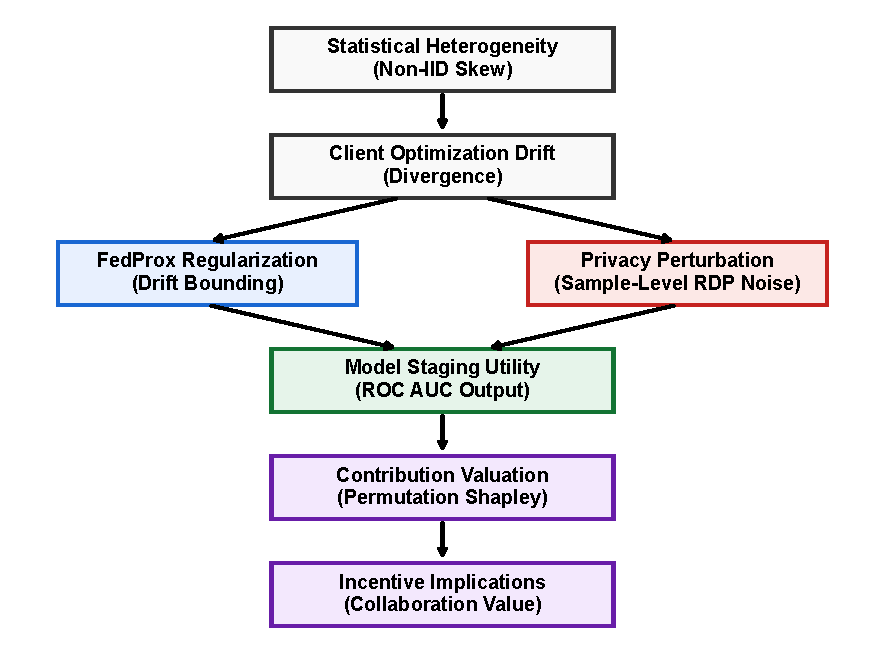
\includegraphics[width=\columnwidth]{figures/figure1_conceptual_map.pdf}
    \caption{Conceptual model of the privacy--heterogeneity--optimization--valuation relationships investigated in this study, tracking variables from data skew to client optimization drift, proximal stabilization, privacy perturbation, staging utility, and collaborative incentive implications.}
    \label{fig:conceptual_map}
\end{figure}

The remainder of this manuscript is organised as follows. Section II reviews related work, Sections III--IV give the system model and methodology, Section V describes both cohorts and the preprocessing, and Section VI the protocol. Section VII presents the primary evaluation on the 19 real hospitals of PCa-19, Section VIII the secondary evaluation on TCGA-PRAD, and the remaining sections discuss limitations, future work and conclusions.

\section{Related Work}



\subsection{Federated Learning for Healthcare}
Cross-silo federated learning has attracted significant interest in clinical AI due to its ability to train models across institutions without direct data sharing \cite{Rieke2020DigitalHealth, Sheller2020MedicineFL, Li2021SurveyFLMedical}. Clinical studies have applied FL to tasks such as brain tumor segmentation, medical imaging, rare cancer research, and tabular clinical risk prediction \cite{Pati2022GFLMedical}. Recently, federated transfer learning has been applied to transfer prognostic models across related cancers under differential privacy \cite{Wen2025Federated}, and decentralized networks have been developed to model pan-cancer survival using clinical-protein sequences \cite{Chai2024AdFed}. To facilitate standardized implementations of these multi-modal models, benchmarks such as FedMultimodal have been established to provide unified recipes for processing multi-site clinical and genomic features \cite{feng2023fedmultimodal}. Tabular databases containing demographic variables, lab values, and genomic markers are highly sensitive, and institutional boundaries prevent their aggregation. While early work assumed identical client data distributions, clinical datasets exhibit severe statistical skew due to differences in patient demographics, diagnostics, and regional pathology characteristics \cite{Kairouz2021FLAdvances, Yang2019ConceptFL}.

\subsection{Non-IID Optimization and Client Drift}
When local datasets are non-IID, the local optimization objectives of clinical clients diverge. Standard Federated Averaging (FedAvg) aggregates updates by computing weighted averages of client parameters \cite{McMahan2017FedAvg}. However, client drift causes local updates to guide parameters away from the global optimum, slowing convergence and reducing utility \cite{Zhao2018NonIID, Wang2021FieldGuide}. To mitigate drift, FedProx adds a proximal regularization term to the local loss, penalizing deviations from the global model \cite{Li2020FedProx}. Alternative approaches like SCAFFOLD use control variates to correct drift, but increase communication overhead by transmitting auxiliary parameters \cite{Karimireddy2020Scaffold}; adaptive server optimisers such as FedAdam apply Adam to the averaged update \cite{Reddi2021FedOpt}, and FedNova normalises updates by the number of local steps \cite{Wang2020FedNova}.

\subsection{Differential Privacy and Rényi DP}
Exposing model weights to a coordinator introduces privacy risks, as membership inference and model inversion attacks can reconstruct patient information. Differential Privacy (DP) provides mathematical guarantees against such leakage \cite{Dwork2008DPSurvey, Dwork2006CalibratingNoise}. DP-SGD applies gradient clipping to limit the influence of individual records, followed by Gaussian noise addition to perturb the aggregated update \cite{Abadi2016DPSGD}. Tracking privacy leakage across communication rounds requires advanced composition methods. Rényi Differential Privacy (RDP) provides tight composition bounds for the Gaussian mechanism, making it suitable for multi-round federated training \cite{Mironov2017RDP, Mironov2019SampledGaussian}. Recent work has extended these mechanisms to handle across-silo user-level differential privacy, guaranteeing that an entire hospital's dataset remains protected against aggregation leaks \cite{Kato2024ULDP}. Furthermore, adaptive weight-based differential privacy (AWDP-FL) has been proposed to dynamically adjust gradient clipping thresholds based on neural network layers, minimizing the utility loss commonly associated with static clipping \cite{Chen2024AWDP}.

\subsection{Client Contribution Valuation}
To keep clinical federations stable, hospitals' contributions must be valued, for example to reward participation \cite{Kazlouski2025HospitalParticipation, Lyu2020FairnessFL}. Leave-One-Out (LOO) methods assess a client's marginal value by comparing global performance with and without that client \cite{Ghorbani2019DataShapley}; LOO ignores synergies between clients and assigns near-zero value to redundant ones. The Shapley value \cite{Shapley1953} averages marginal contributions over all coalitions and is the unique value satisfying efficiency, symmetry, null player and additivity; it has been adapted to data valuation \cite{Ghorbani2019DataShapley, Jia2019KNNShapley, Ghorbani2020NeuronShapley} and to federated clients \cite{Song2019BlockchainFL, Wei2020DataValuation}. Exact Shapley values need a model for each of the $2^K$ coalitions, so federated valuation either samples coalitions \cite{Maleki2013Bounding, Jia2020EfficientShapley} or reconstructs coalition models from the updates of a single training run instead of retraining them \cite{Song2019BlockchainFL, Wei2020DataValuation, Liu2022GTG}. Valuation under privacy constraints is less studied. Zhou \emph{et al.}\ \cite{Zhou2025Data} show that with independent DP noise the uncertainty of data values grows with the estimation budget, and that re-using already released private gradients (correlated noise) avoids this at no extra privacy cost. To improve efficiency, VerFedSV values feature contributions in vertical federated learning \cite{Fan2024VerFedSV}, and threshold KNN-Shapley achieves linear-time valuation with native differential privacy \cite{wang2023threshold}.

\subsection{Membership Inference Attacks in Clinical AI}
While differential privacy provides formal mathematical bounds, empirical privacy audits are needed to measure practical resistance to leakage. Membership Inference Attacks (MIA) aim to determine whether a specific patient record was used in training \cite{Shokri2017MIA}. In clinical applications, the prediction confidence difference between members and non-members serves as an information leak channel. Noise calibration under DP aims to obfuscate this confidence gap, reducing attacker advantage to random guess levels. Recent surveys categorize these attacks into loss-based, shadow-model, and decision-boundary strategies, analyzing diverse countermeasures across federated settings \cite{Bai2025MIA}. Moreover, advanced attacks like FedMIA have demonstrated that adversaries can exploit updates across multiple communication rounds to execute multi-stage inference attacks, highlighting the necessity of robust privacy audits beyond static confidence threshold evaluations \cite{Zhu2025FedMIA}.

\subsection{Research Gap Analysis}
Prior works have typically evaluated heterogeneity, differential privacy, personalization, and contribution valuation as isolated components. The multi-dimensional interactions between these constraints remain under-studied. For instance, the impact of DP noise on game-theoretic client rankings under heterogeneous skews has not been systematically characterized. This study addresses this gap. Table \ref{tab:lit_comparison} contrasts our approach with existing literature.

\begin{table*}[t]
\caption{Comparison of Our Approach with Existing Federated Learning Literature}
\centering
\resizebox{\textwidth}{!}{
\begin{tabular}{lcccccccc}
\toprule
Study & Clinical FL & Non-IID Skew & FedProx & DP & PFL & Shapley & MIA & Privacy $\times$ Heterogeneity \\
\midrule
McMahan et al. \cite{McMahan2017FedAvg} & Yes & Yes & No & No & No & No & No & No \\
Li et al. \cite{Li2020FedProx} & Yes & Yes & Yes & No & No & No & No & No \\
Abadi et al. \cite{Abadi2016DPSGD} & No & No & No & Yes & No & No & No & No \\
Ghorbani et al. \cite{Ghorbani2019DataShapley} & No & No & No & No & No & Yes & No & No \\
Kazlouski et al. \cite{Kazlouski2025HospitalParticipation} & Yes & Yes (real sites) & No & No & No & No & No & No \\
Liu et al. (GTG-Shapley) \cite{Liu2022GTG} & No & Yes & No & No & No & Yes & No & No \\
Zhou et al. \cite{Zhou2025Data} & No & No & No & Yes & No & Yes & No & No \\
\textbf{Ours, PCa-19 (same 19 hospitals)} & \textbf{Yes} & \textbf{Yes (real sites)} & \textbf{Yes} & \textbf{Yes} & \textbf{Yes} & \textbf{Yes (OSA)} & \textbf{Yes} & \textbf{Yes} \\
\textbf{Ours (DP-FPS)} & \textbf{Yes} & \textbf{Yes} & \textbf{Yes} & \textbf{Yes} & \textbf{Yes} & \textbf{Yes} & \textbf{Yes} & \textbf{Yes} \\
\bottomrule
\end{tabular}
}
\label{tab:lit_comparison}
\end{table*}

\section{System Model and Problem Formulation}
Consider a federated network of $K$ clinical clients and a central coordinator.
Each client $k \in \{1, \dots, K\}$ holds a private dataset $D_k = \{(x_{i,k}, y_{i,k})\}_{i=1}^{n_k}$, where $x_{i,k} \in \mathbb{R}^d$ is a clinical feature vector and $y_{i,k} \in \{0, 1\}$ is the pathologic staging target (1 = T3/T4). Let $n = \sum_{k=1}^K n_k$.

The global objective is
\begin{equation}
\min_w F(w) = \sum_{k=1}^K \frac{n_k}{n} F_k(w),
\end{equation}
where $F_k(w) = \frac{1}{n_k} \sum_{i=1}^{n_k} \ell(w; x_{i,k}, y_{i,k}) + \frac{\lambda}{2}\|w\|_2^2$. Under FedAvg, each client performs $E$ local epochs of gradient descent from the current global model and the server averages the results:
\begin{equation}
w^{t+1} = \sum_{k=1}^K \frac{n_k}{n} w_k^{t+1}.
\end{equation}
FedProx adds a proximal term to the local objective,
\begin{equation}
h_k(w; w^t) = F_k(w) + \frac{\mu}{2} \|w - w^t\|_2^2 ,
\end{equation}
which limits how far local models move away from $w^t$ ($\mu=0$ recovers FedAvg).

Local gradients are clipped and perturbed with Gaussian noise calibrated by a Rényi-DP accountant. Client contributions are measured with the Shapley value of the utility $v(S)$, the test AUC of the FedAvg model trained on coalition $S$. The architecture is shown in Fig.~\ref{fig:architecture}.

\begin{figure*}[!t]
    \centering
    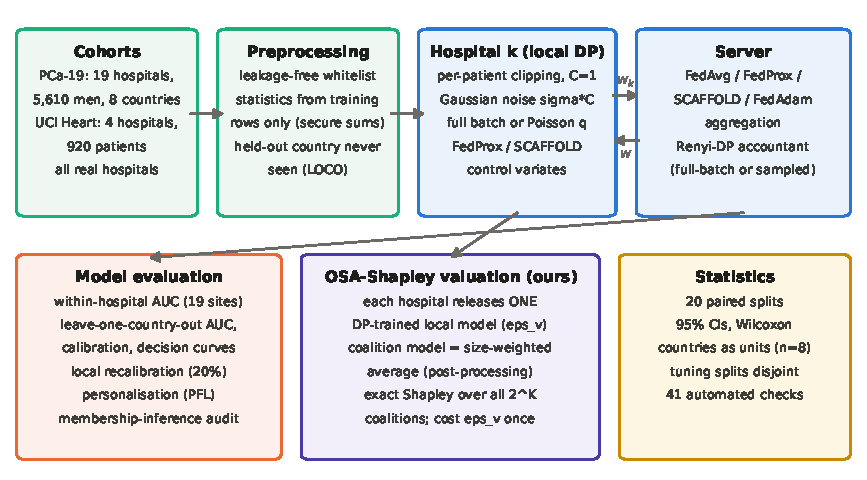
\includegraphics[width=0.7\textwidth]{figures/figure2_architecture.pdf}
    \caption{Experimental system architecture of the DP-FPS clinical federated system: client-level preprocessing, local gradient clipping and RDP-calibrated noise, FedProx aggregation, and post-training Shapley valuation.}
    \label{fig:architecture}
\end{figure*}

\section{Mathematical Methodology}

\subsection{Classification Model}
Staging is modelled with logistic regression with an intercept,
\begin{equation}
p_i = \sigma(z_i) = \frac{1}{1 + e^{-z_i}}, \qquad z_i = x_i^T w + b,
\end{equation}
trained on binary cross-entropy $\ell(w; x_i, y_i) = - [y_i \ln p_i + (1 - y_i) \ln(1 - p_i)]$ with a small $L_2$ penalty ($\lambda = 10^{-3}$).

\subsection{FedProx Local Optimization}
At round $t$ client $k$ starts from $w^t$ and performs $E$ full-batch steps
\begin{equation}
w_k^{t, \tau+1} = w_k^{t, \tau} - \eta \left( \nabla F_k(w_k^{t, \tau}) + \mu (w_k^{t, \tau} - w^t) \right).
\end{equation}
We measure client drift, for both FedAvg and FedProx, as
\begin{equation}
\bar d = \frac{1}{T}\sum_{t=1}^{T} \frac{1}{K}\sum_{k=1}^{K} \big\| w_k^{t} - w^{t-1} \big\|_2 ,
\label{eq:drift}
\end{equation}
the distance between each local model after local training and the global model it started from.

\subsection{Rényi Differential Privacy and Sensitivity Analysis}

\subsubsection{Privacy Unit and Adjacency}
We use add/remove adjacency of single records, $D \sim D' \iff |D \triangle D'| = 1$. Because the analysis cohort keeps exactly one primary-tumour sample per patient (Section~\ref{sec:data}), a record is a patient and the guarantee is patient-level for this cohort.

Each per-sample gradient is clipped to $L_2$ norm $C$,
\begin{equation}
\bar{g}_i = g_i / \max\left(1, \frac{\|g_i\|_2}{C}\right),
\end{equation}
so adding or removing one patient changes the summed gradient by at most $C$. The released (noisy) gradient is
\begin{equation}
\tilde{g} = \frac{1}{n_k}\Big(\sum_{i=1}^{n_k} \bar{g}_i + z\Big), \quad z \sim \mathcal{N}\left(0, \sigma^2 C^2 I\right),
\end{equation}
i.e.\ a Gaussian mechanism with noise multiplier $\sigma$ on a sum query of sensitivity $C$ (client sizes $n_k$ are treated as public). The $L_2$ and proximal terms do not access data and are post-processing.

\subsubsection{Rényi DP Composition}
Updates are full-batch (sampling rate $q=1$), so no subsampling amplification is claimed. A Gaussian mechanism with multiplier $\sigma$ satisfies RDP of order $\alpha>1$ with $\epsilon_{RDP}(\alpha) = \alpha/(2\sigma^2)$. Every patient participates in each of the $N = T \times E$ local steps of its own client, and clients hold disjoint patients, so
\begin{equation}
\epsilon = \min_{\alpha \in \mathcal{A}} \left\{ N \cdot \frac{\alpha}{2 \sigma^2} + \frac{\ln(1/\delta)}{\alpha - 1} \right\},
\end{equation}
with a dense order grid $\mathcal{A}$ (1.1--4096). The accountant agrees with the closed-form optimum $\rho + 2\sqrt{\rho \ln(1/\delta)}$, $\rho = N/(2\sigma^2)$, to within 0.01\% and is never below it. For $N=100$ and $\delta=10^{-5}$ the calibrated multipliers are $\sigma = \sigmaTen, \sigmaFive, \sigmaTwo, \sigmaOne, \sigmaHalf$ for $\varepsilon = 10, 5, 2, 1, 0.5$.

\subsubsection{Subsampled Accounting}
As an alternative we also train with Poisson subsampling: in every local step each patient is included independently with probability $q<1$, the clipped gradients of the included patients are summed, noise $\mathcal{N}(0,\sigma^2C^2I)$ is added and the sum is divided by the \emph{expected} batch size $q\,n_k$; $1/q$ steps make one epoch, so $N = T\,E/q$. One step is then a sampled Gaussian mechanism, whose RDP at integer order $\alpha$ is \cite{Mironov2019SampledGaussian, Zhu2019Poisson, Wang2019SubsampledRDP}
\begin{equation}
\epsilon_{RDP}(\alpha) = \frac{1}{\alpha-1}\ln \sum_{j=0}^{\alpha} \binom{\alpha}{j} (1-q)^{\alpha-j} q^{j} \exp\!\Big(\frac{j^2-j}{2\sigma^2}\Big),
\end{equation}
composed over the $N$ steps and converted as above (orders 2--1024). For $q=1$ it reduces to $\alpha/(2\sigma^2)$. Our implementation matches a numerical evaluation of the Rényi divergence to $10^{-13}$ and reproduces the value $\varepsilon \approx 1.26$ reported by Abadi \emph{et al.}\ \cite{Abadi2016DPSGD} for $q=0.01$, $\sigma=4$, $10{,}000$ steps and $\delta=10^{-5}$. Subsampling lowers the noise multiplier required for a given $\varepsilon$ (privacy amplification \cite{Balle2018Amplification}) at the price of more, smaller-batch steps; whether this improves utility is an empirical question (Section~\ref{sec:p19_subsampling}).

\subsection{Exact Shapley Valuation}
The Shapley value of client $k$ is
\begin{equation}
\phi_k = \sum_{S \subseteq \mathcal{N} \setminus \{k\}} \frac{|S|!(K - |S| - 1)!}{K!} \left[ v(S \cup \{k\}) - v(S) \right],
\end{equation}
with $v(\emptyset)=0.5$. We compute it \emph{exactly} by training all $2^K-1$ coalitions (vectorised across coalitions; numerically identical to separate training runs) for $K \le 10$, so no Monte-Carlo error confounds the effect of DP noise. Leave-one-out (LOO) is $v(\mathcal{N}) - v(\mathcal{N}\setminus\{k\})$. Under DP every coalition run draws independent noise. Note that this \emph{retraining} approach releases $2^{K-1}$ privately trained models that involve each hospital; by composition, its total privacy loss is far larger than the per-run $\varepsilon$ (for $K=10$, $N=100$ and a per-run $\varepsilon=1$ it is $\varepsilon\approx\trueEpsOne$; Table~\ref{tab:osa}). We report it because it is the standard way to study valuation under DP, and contrast it with the privacy-honest estimator below.

\subsection{Privacy-Honest Valuation: OSA-Shapley}
\label{sec:osa}
We propose to value hospitals with \emph{one-shot-averaging Shapley} (OSA-Shapley), which spends the privacy budget once:
\begin{enumerate}
\item Each hospital $k$ releases one logistic-regression model $\hat w_k$ trained locally by DP gradient descent at valuation budget $\varepsilon_v$ (\osaSteps{} full-batch steps, per-patient clipping $C=1$, Gaussian noise calibrated with the accountant above). The released model is the average of the iterates of the second half of training, which damps the injected noise.
\item The server forms the model of every coalition as the size-weighted average $w_S = \sum_{k\in S} (n_k/n_S)\,\hat w_k$. For a convex model trained to convergence this one-shot average approximates the FedAvg solution of the coalition; the base paper itself trains its federated models this way.
\item $v(S)$ is the AUC of $w_S$ on the server's reference set, and exact Shapley values follow from all $2^K-1$ utilities by vectorised bitmask summation.
\end{enumerate}
\emph{Privacy.} Steps 2--3 only post-process the $K$ released models, so by the post-processing property of DP the valuation of \emph{all} coalitions is $(\varepsilon_v,\delta)$-DP for every patient, independently of $K$; if it is released together with the training run, the two budgets compose. \emph{Noise.} Every coalition shares the same released models, so the injected noise is common to all coalitions and largely cancels in marginal contributions. This is the mechanism that Zhou \emph{et al.}\ \cite{Zhou2025Data} exploit by re-using released private gradients, here realised through model reconstruction in the spirit of \cite{Song2019BlockchainFL, Wei2020DataValuation, Liu2022GTG}. \emph{Cost.} Only $K$ local trainings are needed, and the $2^K$ evaluations are cheap: exact Shapley values for all 19 PCa-19 hospitals ($524{,}287$ coalitions) take about a minute on one CPU core. The number of local steps was chosen on four tuning splits that are disjoint from the evaluation splits.

\subsubsection{Ranking Stability Metrics}
For each partition and DP noise realisation $r$ we compare the DP Shapley ranking with the no-DP ranking of the same partition using Spearman's $\rho$, the rank-reversal rate $RR = \frac{1}{K}\sum_k \mathbb{I}(\mathrm{rank}^{DP}_k \neq \mathrm{rank}^{noDP}_k)$, and the top-contributor stability
\begin{equation}
TS = \frac{1}{R} \sum_{r=1}^{R} \mathbb{I}\big(\arg\max_k \phi^{DP}_{k,r} = \arg\max_k \phi^{noDP}_{k}\big),
\end{equation}
whose chance level is $1/K$. (An earlier version averaged $\mathbb{I}(\mathrm{rank}^{DP}_{k,r}=1)$ over clients, which equals $1/K$ by construction for every configuration.)

\subsection{Membership Inference Attack Formulation}
We audit empirical leakage with a confidence-threshold membership-inference attack. The score of a record is the model's confidence in its true label, $s_i = y_i p_i + (1 - y_i)(1 - p_i)$. Members (training patients) are subsampled to the number of non-members (test patients) and the attack is summarised by its ROC AUC. As a positive control, the same attack is applied to a deliberately over-fitted model (200 random noise features, no regularisation).

\subsection{Domain Shift Formulations}
Robustness is probed with synthetic perturbations of the held-out split: covariate shift scales each numeric feature by $\beta_j \sim U(1-0.25s, 1+0.25s)$ and adds $\mathcal{N}(0, (0.5s)^2)$ noise; concept shift flips a fraction $\min(0.25s, 0.5)$ of labels, for severity $s$.

\subsection{Statistical Analysis}
Every experiment is repeated over 20 seeds. A seed re-draws the stratified 80/20 split, the client partition, model noise and DP noise, so seed-to-seed variation covers all sources of randomness. We report means with $t$-based 95\% confidence intervals over seeds. Comparisons between methods are \emph{paired} by seed; we report the mean paired difference with its 95\% CI and a two-sided Wilcoxon signed-rank test, and call a difference significant only if its CI excludes zero. For ranking stability we additionally apply a one-sided Wilcoxon test of $d_i = \rho_i - 0.90 < 0$, where $\rho_i$ is the seed-level Spearman correlation. Per-client AUCs are averaged only over clients whose local test split contains both classes (macro AUC); we do not pool predictions of different local models, because pooling rewards each model for learning its own client's base rate.

\section{Datasets and Preprocessing}
\label{sec:data}

\subsection{PCa-19: The Base Paper's 19-Hospital Cohort}
PCa-19 is the patient-level collection used by the base paper, released in the authors' public repository (MIT licence) \cite{Kazlouski2025HospitalParticipation}. The authors harmonised it from the supplementary files of 19 peer-reviewed prostate-cancer studies. It contains \pNineN{} men from \pNineHosp{} hospitals (Table~\ref{tab:pca19_cohort}); \pNinePos{} (\pNinePrev\%) have clinically significant cancer (csPCa, ISUP grade group $\geq 2$ at biopsy), ranging from \pNinePrevLo\% to \pNinePrevHi\% per hospital. The base paper's text states nine countries, but its Table~I and the released data contain eight (Spain, South Korea, Germany, China, USA, Netherlands, Italy, UK); we use the released data unchanged. Every variable is available before biopsy: age, PSA, prostate volume (PV) and the highest PI-RADS score. (A 5-$\alpha$-reductase-inhibitor flag is 0 for all patients and is not used.) Our feature set is age, $\log$ PSA, $\log$ PV and indicators for PI-RADS 3, 4 and 5. The logarithms keep the extreme PSA values of one hospital (median 277~ng/mL) from dominating, and standardisation statistics are computed from training rows only. For the reproduction of the authors' protocol we use their exact Ettala and Noh variables.

\begin{table}[t]
\caption{PCa-19: the base paper's 19-hospital pre-biopsy cohort (5{,}610 men). csPCa = ISUP grade group $\geq 2$ at biopsy; medians of age (years), PSA (ng/mL) and prostate volume (mL); PI-RADS $\geq 4$ in \%.}
\centering\scriptsize
\setlength{\tabcolsep}{3pt}
\begin{tabular}{llrrrrrr}
\toprule
Hosp. & Country & $n$ & csPCa\% & Age & PSA & Vol. & PI-RADS$\geq$4 \\
\midrule
de1 & Germany & 763 & 43 & 65 & 8.0 & 47 & 74 \\
es7 & Spain & 711 & 50 & 67 & 7.6 & 53 & 55 \\
kr2 & South Korea & 590 & 38 & 68 & 7.0 & 42 & 72 \\
ch2 & China & 530 & 33 & 67 & 10.3 & 41 & 42 \\
kr1 & South Korea & 406 & 25 & 64 & 6.8 & 36 & 28 \\
es6 & Spain & 346 & 43 & 69 & 7.6 & 52 & 78 \\
ch1 & China & 312 & 27 & 66 & 9.7 & 45 & 43 \\
us2 & USA & 310 & 48 & 65 & 7.3 & 46 & 82 \\
us1 & USA & 280 & 45 & 62 & 5.5 & 45 & 62 \\
nl & Netherlands & 266 & 26 & 67 & 11.1 & 56 & 36 \\
it & Italy & 218 & 12 & 65 & 8.0 & 54 & 38 \\
es4 & Spain & 200 & 34 & 69 & 7.6 & 55 & 56 \\
es5 & Spain & 200 & 47 & 70 & 10.6 & 56 & 80 \\
de2 & Germany & 162 & 47 & 65 & 6.5 & 40 & 70 \\
gb & United Kingdom & 133 & 29 & 64 & 7.6 & 45 & 48 \\
es1 & Spain & 79 & 42 & 69 & 6.3 & 61 & 97 \\
es8 & Spain & 58 & 38 & 70 & 6.5 & 56 & 81 \\
es3 & Spain & 30 & 60 & 69 & 9.0 & 50 & 97 \\
es2 & Spain & 16 & 38 & 64 & 277.0 & 81 & 69 \\
\bottomrule
\end{tabular}
\label{tab:pca19_cohort}
\end{table}


\subsection{TCGA-PRAD Cohorts}
We use the clinical, survival and RPPA protein data of TCGA-PRAD \cite{TCGA2015PRAD}. The clinical file contains \nRaw{} sample records from \nRawPatients{} patients, including normal-tissue and metastatic samples. We keep primary-tumour samples (barcode type \texttt{-01}) with a recorded pathologic T stage and one sample per patient, giving a \emph{clinical cohort} of \nClinical{} patients (\nClinicalPos{} T3/T4). Restricting to patients with protein data (\nProteinSamples{} samples) gives the \emph{matched cohort} of \nMatched{} patients (\nMatchedPos{} T3/T4), used for all DP-FPS experiments so that clinical-only and multimodal models are compared on identical patients. Each seed splits it 80/20 into \nTrain{} training and \nTest{} test patients.

\subsection{Feature Whitelist and Leakage Control}
Features are taken from an explicit whitelist: age, race, ethnicity, clinical T and M stage, prior malignancy (pre-operative), plus primary and secondary Gleason pattern, Gleason sum and pathologic N stage (post-surgical pathology). After one-hot encoding (reference level dropped) this gives \nFeatFull{} features (\nFeatPreop{} pre-operative). Identifiers (sample, case, treatment and pathology-report IDs), record timestamps, and outcome or follow-up variables (vital status, days to last follow-up, treatment fields) are excluded; an earlier version of the pipeline admitted about 1{,}650 one-hot columns built from such per-patient identifiers. Gleason pattern and pathologic N come from the same prostatectomy report as the pathologic T label, so they are strong but label-adjacent predictors; we therefore also report a pre-operative-only model. Imputation (median, or an explicit \emph{Unknown} level), scaling and encoding are fitted on training rows only.

For the multimodal ablation, the \nProteinRaw{} RPPA targets are filtered to the \nProteinKept{} with at most 30\% missing values, median-imputed, standardised and reduced by PCA to 95\% explained variance, all fitted on the training split (about 115 components, depending on the split; \nPCAll{} if PCA were fitted on all \nMatched{} patients).

\subsection{Client Partitions}
\emph{Real sites.} For the replication of the base paper we use the TCGA tissue-source site as the hospital: the \nSites{} sites with at least 20 patients (\nSiteTotal{} patients) are clients, each split 80/20 (stratified when possible); the \nExternal{} patients of smaller sites never train and act as external free-riders. Preprocessing statistics are shared across sites (as obtainable by secure aggregation).

\emph{Dirichlet label skew.} For DP-FPS we draw, for each class, client proportions from $\mathrm{Dir}(\alpha)$ and apply the \emph{same} proportions to the training and the test split, so every client has a local test set with its own label skew; $\alpha \in \{100, 10, 1, 0.5, 0.1\}$ (smaller = more heterogeneous). Unless stated otherwise $K=3$.

\subsection{Survival Events}
The matched cohort contains only \nEvents{} deaths (\nEventsTrain{} in the training and \nEventsTest{} in the test split for the reference seed; \nEventsAll{} deaths over all \nRaw{} records). Survival modelling is therefore not evaluated.

\section{Experimental Protocol}
Unless stated otherwise: $T=20$ rounds, $E=5$ local epochs ($N=100$ steps), learning rate $\eta=0.5$, $\lambda=10^{-3}$, $\mu=0.5$, $C=1$, $\delta=10^{-5}$, 20 seeds (Table~\ref{tab:protocol}). The optimiser settings were chosen by cross-validation of the centralised NumPy model, whose AUC then matches scikit-learn's logistic regression (\cvFull{} vs \cvSkFull{}, Table~\ref{tab:centralized}).

\begin{table}[ht]
\caption{Experimental Protocol}
\centering
\footnotesize
\begin{tabular}{ll}
\toprule
Parameter & Value \\
\midrule
Raw records / patients & \nRaw{} / \nRawPatients{} \\
Clinical cohort (1 sample/patient) & \nClinical{} \\
Matched cohort (train/test) & \nMatched{} (\nTrain{}/\nTest{}) \\
Clinical features (full / pre-op) & \nFeatFull{} / \nFeatPreop{} \\
Proteins (ablation) & \nProteinRaw{} $\to$ \nProteinKept{} $\to$ PCA 95\% \\
Rounds $T$ / local epochs $E$ & 20 / 5 \\
Learning rate $\eta$ / $L_2$ $\lambda$ & 0.5 / $10^{-3}$ \\
FedProx $\mu$ & 0.5 \\
Clipping $C$ / $\delta$ & 1.0 / $10^{-5}$ \\
Seeds per experiment & 20 \\
\bottomrule
\end{tabular}
\label{tab:protocol}
\end{table}

\section{Results}
\label{sec:results}
All results use real hospitals as released: the 19 PCa-19 hospitals and, in Section~\ref{sec:heart}, the four heart-disease hospitals. We first summarise the federation that is valued (Section~\ref{sec:federation}); its full analysis is in Supplementary Section~\ref{S-sec:pca19_more}. We then turn to valuation under DP (Sections~\ref{sec:p19_retrain}--\ref{sec:heart}).

\subsection{The Federation Being Valued}
\label{sec:federation}
Our re-implementation of the base paper's protocol reproduces the authors' released code to within $1.2\times10^{-14}$ for both of their calculators (Supplementary Section~\ref{S-sec:p19_repro}), and its sustainability finding holds under our protocol: joining brings no significant average gain over local training (FL$-$LOC $=\pDFLminusLOC$), a free-rider obtains almost the same model (FR$-$FL $=\pDFRminusFL$), and federated training matches pooled training (CEN$-$FL $=\pDCENminusFL$). For this seven-parameter, regularised logistic calculator trained on \pNineN{} patients, DP changes the mean per-hospital AUC by only $\pDpLossHalf$ even at $\varepsilon=0.5$. We do not generalise this: the cost of a given $\varepsilon$ depends strongly on the model and the amount of data, and for a federated MLP the same budgets perturb the released models far more (Section~\ref{sec:p19_mlp}). Discrimination transports to held-out countries, but calibration does not (observed/expected ratios \pOeMin--\pOeMax); an intercept update on 20\% of a new country's patients, which is common clinical practice for risk calculators anyway, reduces $|\log\mathrm{O/E}|$ from \pRecalOeRaw{} to \pRecalOeInt{} (Supplementary Section~\ref{S-sec:p19_loco}).

\subsection{Retraining-Based Valuation under DP}
\label{sec:p19_retrain}
Following standard practice, we first retrain every coalition with DP at a per-run $\varepsilon$ and compute exact Shapley values over the ten largest hospitals (1{,}023 coalitions). Their agreement with the non-private ranking falls from Spearman $\rho=\pShRhoTen$ at $\varepsilon=10$ to \pShRhoTwo{} at $\varepsilon=2$ and \pShRhoHalf{} at $\varepsilon=0.5$ (original splits, against the no-DP ranking; Table~\ref{S-tab:osa} repeats this on the held-out splits against exact Shapley), although the federation's AUC changes by less than 0.01 over this range. Leave-one-out values are near zero for every hospital and cannot separate contributors (Spearman with Shapley \pShLooRho). These results ignore the cost of the valuation itself.

\subsection{Valuation at an Honest Privacy Budget}
\label{sec:p19_osa}
Table~\ref{S-tab:osa} makes the real cost of retraining explicit: with ten hospitals each hospital joins 512 private training runs, so a per-run $\varepsilon$ of 10, 5 or 1 corresponds to a total $\varepsilon$ of about \trueEpsTen{}, \trueEpsFive{} and \trueEpsOne{} per hospital. When the total budget is held at the stated $\varepsilon$ (\emph{budget-matched} retraining), every run needs much more noise and the ranking is lost: Spearman $\rho$ with the exact non-private Shapley values falls to \bmRhoTen{} at $\varepsilon=10$ and \bmRhoOne{} at $\varepsilon=1$.

OSA-Shapley (Section~\ref{sec:osa}) spends the budget once. Without DP it reproduces the retraining Shapley ranking almost exactly ($\rho=\osaNoDP$), and under DP it keeps $\rho=\osaRhoTen$ at $\varepsilon=10$, \osaRhoTwo{} at $\varepsilon=2$, \osaRhoOne{} at $\varepsilon=1$ and \osaRhoHalf{} at $\varepsilon=0.5$ (Table~\ref{S-tab:osa}; evaluated on 20 splits that were not used to choose its single hyper-parameter). At equal privacy it beats retraining by $\osaVsBmTwo$ in $\rho$ at $\varepsilon=2$. At $\varepsilon=2$ it matches per-run retraining ($\osaVsPrTwo$), which spends 28--42 times more privacy. Because no coalition needs training, exact valuation of all 19 hospitals is feasible: the OSA ranking computed with DP agrees with the non-private one at $\rho=\osaNineRhoFive$ ($\varepsilon=5$) and \osaNineRhoOne{} ($\varepsilon=1$).


\subsection{Against Valuations that Also Cost the Budget Once}
\label{sec:p19_post}
The fair competitors are the reconstruction methods MR and OR, which post-process the DP-FedAvg run (Section~\ref{sec:osa}). Table~\ref{S-tab:osa_post} and Fig.~\ref{S-fig:osa} compare them on the same splits. For the ten largest hospitals, OSA-Shapley is more accurate than exact MR, the upper bound for GTG-Shapley, at every privacy level: $\rho$ \osaRhoTwo{} vs \mrRhoTwo{} at $\varepsilon=2$ (difference \osaVsMrTwo) and \osaRhoOne{} vs \mrRhoOne{} at $\varepsilon=1$ (\osaVsMrOne). It also beats OR by \osaVsOrTwo{} at $\varepsilon=2$. The gap is already present without DP ($\rho$ \osaNoDP{} vs \mrRhoNoDP), so it comes from the coalition proxy rather than from the noise.


\subsection{Is OSA-Shapley Worth It? Cheap Proxies}
\label{sec:p19_proxies}
A federation could avoid a valuation protocol altogether and credit hospitals by what they can share cheaply. Table~\ref{tab:proxies} compares these proxies with OSA-Shapley against the same exact non-private reference. For the ten largest hospitals, hospital size, the number of cancer cases and the similarity of summary statistics to the pooled ones carry almost no information about contribution ($\rho$ \pxLSizeNoDP, \pxLPosNoDP{} and \pxLStatNoDP; OSA$-$size $=\pxdLSizeTwo$ at $\varepsilon=2$). They also cannot detect a hospital with useless data, because random labels change neither its size nor its prevalence (0\% of splits). Hospitals here differ in case mix, not only in size, and their marginal value depends on what the other hospitals already provide. An AUC that each hospital reports for its own model is unverifiable and agrees poorly with the ranking ($\rho=\pxLOwnTwo$ at $\varepsilon=2$).

Proxies built on a released model behave differently. Once each hospital has released one DP model, as OSA requires, the AUC of that single model on the reference set already ranks the large hospitals well ($\rho=\pxLRefTwo$ at $\varepsilon=2$) and flags the useless hospital. OSA-Shapley is comparable at $\varepsilon=2$ ($\pxdLRefTwo$) and better at $\varepsilon=1$ ($\pxdLRefOne$), where single releases are noisy and averaging over coalitions helps; it also beats the leave-one-out value of the averaged releases by $\pxdLLooTwo$. Both scores use the same releases, so OSA's advantage costs no extra privacy or communication. OSA's values are also Shapley values: they sum to the federation's gain over chance, which a single-model score does not.

On the ten smallest hospitals the picture changes (Table~\ref{tab:proxies}, right). There contribution is driven mainly by data volume, and hospital size alone reaches $\rho=\pxSSizeNoDP$. At $\varepsilon=2$, OSA-Shapley, MR, the single-model score and size agree with the ranking about equally well (OSA$-$size $=\pxdSSizeTwo$, OSA$-$MR $=\pxdSMrTwo$), and at $\varepsilon=1$ none of the DP valuations is better than size.

\begin{table*}[t]
\caption{Is OSA-Shapley worth its cost? Agreement (Spearman $\rho$) of cheap contribution proxies and of privacy-honest valuations with the exact non-private retraining Shapley ranking, on real PCa-19 hospitals (20 held-out splits). \emph{What is shared}: what each hospital must reveal. Proxies that use a model use the same DP releases as OSA-Shapley and therefore cost the same $\varepsilon$; size, counts and statistics are shared without DP. \emph{Useless}: share of splits in which a hospital whose training labels were replaced by random labels (es6) is ranked last at $\varepsilon=2$; a tie for last place does not count.}
\centering\scriptsize
\setlength{\tabcolsep}{4pt}
\begin{tabular}{llccccccc}
\toprule
 & & \multicolumn{4}{c}{Ten largest hospitals} & \multicolumn{3}{c}{Ten smallest hospitals} \\
\cmidrule(lr){3-6}\cmidrule(lr){7-9}
Contribution score & What is shared & no DP & $\varepsilon=2$ & $\varepsilon=1$ & Useless & no DP & $\varepsilon=2$ & $\varepsilon=1$ \\
\midrule
Hospital size $n_k$ & size (public) & 0.08 & 0.08 & 0.08 & 0\% & 0.74 & 0.74 & 0.74 \\
Number of csPCa cases & one count & 0.02 & 0.02 & 0.02 & 0\% & 0.50 & 0.50 & 0.50 \\
Similarity of summary statistics & feature means, prevalence & \ensuremath{-}0.18 & \ensuremath{-}0.18 & \ensuremath{-}0.18 & 0\% & 0.72 & 0.72 & 0.72 \\
Self-reported local AUC & one AUC (unverifiable) & 0.36 & 0.25 & 0.26 & 100\% & 0.40 & 0.54 & 0.56 \\
Single-model AUC on reference set & one DP model ($\varepsilon$) & 0.93 & 0.85 & 0.71 & 100\% & 0.94 & 0.79 & 0.72 \\
Leave-one-out of averaged models & one DP model ($\varepsilon$) & 0.85 & 0.77 & 0.74 & 0\% & 0.59 & 0.34 & 0.34 \\
OR reconstruction & DP-FedAvg run ($\varepsilon$) & 0.42 & 0.51 & 0.50 & 100\% & 0.79 & 0.74 & 0.59 \\
MR reconstruction (GTG bound) & DP-FedAvg run ($\varepsilon$) & 0.74 & 0.75 & 0.65 & 70\% & 0.86 & 0.78 & 0.74 \\
Retraining, budget-matched & $2^{K-1}$ runs ($\varepsilon$) & -- & 0.18 & 0.10 & 60\% & -- & 0.45 & 0.29 \\
\textbf{OSA-Shapley (ours)} & one DP model ($\varepsilon$) & \textbf{0.96} & \textbf{0.89} & \textbf{0.80} & 100\% & \textbf{0.95} & \textbf{0.79} & \textbf{0.68} \\
\bottomrule
\end{tabular}
\label{tab:proxies}
\end{table*}


\subsection{A Hospital with Useless Data, Removal and Robustness}
\label{sec:p19_robust}
We replaced the training labels of one mid-sized hospital (\corrHosp) by random labels and asked whether each valuation ranks it last (Tables~\ref{tab:proxies} and~\ref{S-tab:osa_robust}). The non-private retraining Shapley values always do (\corrTruth). At $\varepsilon=2$ and $\varepsilon=1$, OSA-Shapley ranks it last in \corrOsaTwo{} and \corrOsaOne{} of splits, MR in \corrMrTwo{} and \corrMrOne, and budget-matched retraining in only \corrBmTwo{} and \corrBmOne; no size- or statistics-based proxy ever does. Sensitivity to the reference-set size and the number of local steps is reported in Table~\ref{S-tab:osa_robust}.

\subsection{A Non-Convex Model}
\label{sec:p19_mlp}
OSA-Shapley assumes that averaging locally trained models approximates the federated model of a coalition, which holds for convex losses. We therefore repeated the comparison with a one-hidden-layer MLP (16 tanh units) trained by FedAvg, with exact non-private retraining Shapley values of the federated MLP as the reference (Table~\ref{S-tab:osa_mlp}). Because averaging the parameters of separately trained networks is fragile, the coalition prediction is the size-weighted average of the members' log-odds (OSA-ens.), which is equally post-processing. Without DP the ensemble variant reproduces the reference ranking well ($\rho=\mlpOsaNoDP$, against \mlpMrNoDP{} for MR). Under DP it loses this advantage: at $\varepsilon=2$ and $\varepsilon=1$ it reaches \mlpOsaTwo{} and \mlpOsaOne{}, whereas MR reaches \mlpMrTwo{} and \mlpMrOne{} (OSA$-$MR $=\mlpOsaVsMrTwo$ at $\varepsilon=2$). A non-linear model trained alone for 200 noisy steps accumulates the DP perturbation, whereas MR's short local updates restart from the shared global model in every round. Budget-matched retraining of the MLP is close to chance ($\rho=\mlpBmTwo$; \mlpBmSeeds{} splits). For non-convex models, reconstruction from the training run is the better privacy-honest valuation.


\subsection{Small Hospitals: Where OSA-Shapley Loses Its Advantage}
\label{sec:p19_small}
To study small silos without simulating any, we value the ten smallest PCa-19 hospitals (\pxSmallMin--\pxSmallMax{} patients; exact non-private retraining Shapley as reference, 20 held-out splits). Without DP, OSA-Shapley is again the most accurate valuation ($\rho=\pxSOsaNoDP$; OSA$-$MR $=\pxdSMrNoDP$). Under DP its advantage disappears: at $\varepsilon=2$ OSA and MR agree with the ranking equally well (\pxSOsaTwo{} and \pxSMrTwo{}; difference $\pxdSMrTwo$), and at $\varepsilon=1$ MR is slightly, not significantly, ahead (\pxdSMrOne). Budget-matched retraining remains far worse ($\rho=\pxSBmTwo$ at $\varepsilon=2$). This is the regime that Proposition~3 predicts: the release of a hospital with a few dozen patients carries noise of order $\sigma/n_k$, whereas reconstruction averages over the federation in every round. With hospitals this small, hospital size is itself a strong proxy (Section~\ref{sec:p19_proxies}), and no privacy-honest valuation improves on it at $\varepsilon \le 1$.


\subsection{A Second Real Federation: Heart Disease}
\label{sec:heart}
Table~\ref{tab:heart} repeats the comparison on the four hospitals of the UCI Heart Disease collection, with OSA-Shapley's PCa-19 hyper-parameters unchanged. Without DP the picture is the same as before: OSA-Shapley recovers the exact ranking best ($\rho=\hrOsaNoDP$, against \hrMrNoDP{} for MR and \hrRefNoDP{} for the single-model score; OSA$-$MR $=\hrdMrNoDP$). Under DP it is not. These hospitals have 98--242 training patients for 21 model parameters, and their contributions are nearly equal (Shapley values \hrPhiMin--\hrPhiMax{} AUC), so the noise of a single release dominates. At $\varepsilon=5$ OSA-Shapley and MR are close (\hrOsaFive{} and \hrMrFive{}); at $\varepsilon=2$ MR is better (\hrMrTwo{} vs \hrOsaTwo{}; OSA$-$MR $=\hrdMrTwo$); and at $\varepsilon=1$ no valuation agrees with the ranking beyond chance. Retraining does not help: with four hospitals its composed cost is modest (a stated $\varepsilon=2$ really costs \hrTrueTwo), yet per-run and budget-matched retraining reach only \hrPrTwo{} and \hrBmTwo{}. Hospital size is anti-correlated with contribution ($\rho=\hrSizeNoDP$): the smallest hospital, Zurich/Basel, contributes most. Released models still detect bad data: OSA-Shapley and the single-model score rank \hrCorrupt{} with random labels last in \hrCOsaTwo{} and \hrCRefTwo{} of splits at $\varepsilon=2$, hospital size in \hrCSizeTwo.

\begin{table}[t]
\caption{Second real federation: the four hospitals of the UCI Heart Disease collection (Cleveland (303), Budapest (294), Zurich/Basel (123), Long Beach VA (200) patients), coronary artery disease, 20 held-out splits. Spearman $\rho$ with the exact non-private retraining Shapley ranking; with four hospitals $\rho$ moves in steps of 0.2. Per-run retraining really costs $\varepsilon\approx16$, 6.1 and 2.9 at a stated 5, 2 and 1. \emph{Useless}: share of splits in which Budapest, given random training labels, is ranked last at $\varepsilon=2$.}
\centering\scriptsize
\setlength{\tabcolsep}{3pt}
\begin{tabular}{lccccc}
\toprule
Contribution score & no DP & $\varepsilon=5$ & $\varepsilon=2$ & $\varepsilon=1$ & Useless \\
\midrule
Hospital size $n_k$ & \ensuremath{-}0.38 & \ensuremath{-}0.38 & \ensuremath{-}0.38 & \ensuremath{-}0.38 & 0\% \\
Similarity of summary statistics & \ensuremath{-}0.38 & \ensuremath{-}0.38 & \ensuremath{-}0.38 & \ensuremath{-}0.38 & 0\% \\
Self-reported local AUC & \ensuremath{-}0.18 & \ensuremath{-}0.17 & \ensuremath{-}0.31 & \ensuremath{-}0.30 & 70\% \\
Single-model AUC on reference set & 0.76 & 0.42 & \ensuremath{-}0.04 & \ensuremath{-}0.34 & 100\% \\
Leave-one-out of averaged models & 0.82 & 0.69 & 0.42 & 0.18 & 85\% \\
OR reconstruction & 0.23 & 0.29 & 0.18 & 0.04 & -- \\
MR reconstruction (GTG bound) & 0.70 & 0.64 & 0.45 & \ensuremath{-}0.35 & -- \\
Retraining, per run & -- & 0.34 & \ensuremath{-}0.09 & \ensuremath{-}0.27 & -- \\
Retraining, budget-matched & -- & \ensuremath{-}0.02 & \ensuremath{-}0.18 & \ensuremath{-}0.15 & -- \\
\textbf{OSA-Shapley (ours)} & \textbf{0.92} & \textbf{0.51} & \textbf{0.15} & \textbf{\ensuremath{-}0.18} & 100\% \\
\bottomrule
\end{tabular}
\label{tab:heart}
\end{table}


\section{A Decision Rule, Tested in Advance}
\label{sec:rule}
\subsection{The Index and the Original Rule}
Supplementary Table~\ref{S-tab:decision} puts the four settings side by side. By Proposition~3 the per-coordinate noise of a release scales as $1/n_k$, so its norm over $p$ parameters scales as $\sqrt p/n_k$; we therefore index a setting by $\nu$, the median number of training patients per hospital divided by $\sqrt p$. In these settings OSA-Shapley won at $\nu=\nuLarge$ (ten largest PCa-19 hospitals) and did not at $\nu\le\nuSmall$ (ten smallest: \nuSmall; heart disease: \nuHeart; MLP: \nuMlp), which suggested a switch-over between $\nu\approx50$ and 100.

\subsection{A Pre-Registered Test}
A threshold read off the same results it explains is not evidence, so we tested it on new conditions. Before running anything, we wrote down the design and six hypotheses and fixed them with a cryptographic hash (Supplementary Section~\ref{S-sec:prereg}); the protocol was registered internally, not on a public registry, and written and run on the same day. Within the ten largest PCa-19 hospitals we lowered $\nu$ in two ways: arm A keeps 60\% to 15\% of every hospital's training patients, and arm B adds 21 to 100 uninformative features; in each condition the reference is the exact non-private retraining Shapley ranking of that condition (Fig.~\ref{fig:nu}, Table~\ref{S-tab:nu_sweep}).

The direction of the rule held, but its threshold did not. As predicted, OSA-Shapley beat MR at $\nu\ge100$ (H1), its advantage shrank with $\nu$ (H3; Spearman correlation \nsSpear{}), both arms agreed in sign at matched $\nu$ (H5), and stronger privacy moved the switch-over to higher $\nu$ (H6). Contrary to H2 and H4, OSA-Shapley kept a significant advantage down to $\nu\approx\nsAFortyFiveNu$ (OSA$-$MR $=\nsAFortyFiveTwo$ at $\varepsilon=2$), tied with MR at $\nu\approx30$--57 when parameters were added, and fell behind only at $\nu\approx\nsASeventeenNu$ (OSA$-$MR $=\nsASeventeenTwo$ at $\varepsilon=2$, $\nsASeventeenOne$ at $\varepsilon=1$). The mean difference changed sign at $\nu\approx\nsCrossTwo$ for $\varepsilon=2$ and between \nsCrossOneMin{} and \nsCrossOneMax{} for $\varepsilon=1$, not between 50 and 100. Two of the six hypotheses therefore failed, and we revise the rule accordingly.

\begin{figure}[!t]
\centering
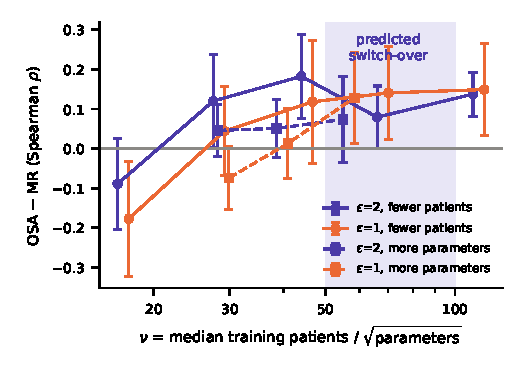
\includegraphics[width=\columnwidth]{figures/figure20_nu_sweep.pdf}
\caption{Pre-registered test: OSA$-$MR (paired difference in Spearman $\rho$ with the exact reference, 95\% CI, 20 splits) as $\nu$ is lowered within the ten largest PCa-19 hospitals, by removing patients (solid) or adding uninformative parameters (dashed). Shaded: the switch-over predicted before the test. Points at the same $\nu$ are offset slightly for legibility.}
\label{fig:nu}
\end{figure}

\subsection{The Revised Rule}
\begin{enumerate}
    \item \emph{Count the cost.} Report the composed $\varepsilon$ of any valuation (Proposition~2) and do not retrain coalitions at a per-run budget; retraining was not accurate in any setting.
    \item \emph{Without DP on the releases} (for example, when model sharing is covered by a data-use agreement), use OSA-Shapley, the most accurate valuation in all four settings ($\rho$ \mlpOsaNoDP--\osaNoDP).
    \item \emph{Under DP with a convex model}, OSA-Shapley is at least as accurate as MR down to $\nu\approx30$ at $\varepsilon=2$ and $\nu\approx40$ at $\varepsilon=1$; below that, use MR, which adds no privacy cost when the federation already trains with DP-FedAvg.
    \item \emph{With a non-convex model}, use MR.
    \item \emph{Check hospital size before using it.} Size matched contribution only where hospitals differed mainly in volume (\pxSSizeTwo{} for the ten smallest PCa-19 hospitals) and failed elsewhere (\pxLSizeTwo{} and \hrSizeTwo). Neither size nor summary statistics can detect bad data; the score of a single released model can.
    \item \emph{Compute both OSA-Shapley and MR when in doubt.} $\nu$ does not explain every case: the heart-disease federation ($\nu=\nuHeart$) favoured MR although the sweep says OSA should be competitive there. Its four hospitals make $\rho$ coarse, and site-specific missing data make some features constant within a hospital, so single-hospital models are poorly determined; both explanations are untested. Disagreement between the two valuations is a sign that the ranking is not resolved at the chosen budget, and with small $\nu$ at $\varepsilon\le1$ coarse credit (equal shares plus screening for bad data) is the honest fallback.
\end{enumerate}


\begin{table*}[t]
\caption{Claim--evidence summary. Verdicts are computed from the result files: `supported' only if the 95\% CI of the paired difference over seeds excludes 0 in the claimed direction; the pre-registered rows are scored by the criteria fixed in advance (Section~\ref{sec:prereg}).}
\centering\scriptsize
\begin{tabular}{p{1.4cm}p{4.2cm}p{8.6cm}p{1.5cm}}
\toprule
Area & Claim & Evidence (mean [95\% CI]) & Verdict \\
\midrule
PCa-19 (19 hospitals) & Joining FL gives hospitals a significant average local gain & FL - LOC (mean per-hospital AUC) = \ensuremath{-}0.005 {[}-0.015, +0.006{]} & not significant \\
PCa-19 (19 hospitals) & Free-riders get (almost) the same model as participants & FR - FL = \ensuremath{-}0.002 {[}-0.002, \ensuremath{-}0.001{]} & supported \\
PCa-19 (19 hospitals) & Federated training matches pooled training & CEN - FL = +0.002 {[}-0.001, +0.004{]} & supported \\
PCa-19 (19 hospitals) & FL beats the published Noh calculator (hospital-averaged AUC) & FL - Noh = \ensuremath{-}0.010 {[}-0.016, \ensuremath{-}0.005{]}; patient-weighted FL 0.856 vs Noh 0.850 & opposite \\
PCa-19 (19 hospitals) & Our re-implementation reproduces the base paper's code exactly & noh: max $|$difference$|$ 1.2e-14 over 5x19 cells (50 repeats); ettala: max $|$difference$|$ 7.8e-15 over 5x19 cells (50 repeats) & supported \\
PCa-19 (19 hospitals) & Federated model transports to unseen countries as well as pooled training & leave-one-country-out, FedAvg - centralised = \ensuremath{-}0.000 {[}-0.001, +0.001{]} (8 countries) & supported \\
PCa-19 (19 hospitals) & DP lowers the calibration slope (predictions more extreme) on held-out countries & slope at $\varepsilon$=5 = 0.81 {[}0.70, 0.92{]} over 8 countries (no DP 1.12) & supported \\
PCa-19 (19 hospitals) & Local recalibration (20\% of a new country) fixes calibration-in-the-large & $|$log O/E$|$ recalibrated - transported = \ensuremath{-}0.193 {[}-0.347, \ensuremath{-}0.038{]} & supported \\
PCa-19 (19 hospitals) & Strong privacy ($\varepsilon$ = 0.5) costs $<$ 0.02 AUC at this scale & FedAvg($\varepsilon$=0.5) - no DP = \ensuremath{-}0.005 {[}-0.011, +0.001{]} & supported \\
PCa-19 (19 hospitals) & FedProx's effect equals halving FedAvg's learning rate & largest $|$FedProx - FedAvg(lr/2)$|$ over 6 privacy levels = 0.0009 AUC; drift reduction 30.8\% & explained by step size \\
PCa-19 (19 hospitals) & Personalisation helps small hospitals ($<$ 100 patients) & PFL - FedProx = +0.039 {[}+0.013, +0.065{]} & supported \\
PCa-19 (19 hospitals) & DP noise destabilises Shapley rankings of real hospitals & 10 hospitals: Spearman 0.94 ($\varepsilon$=10) $\rightarrow$ 0.64 ($\varepsilon$=0.5) & supported \\
PCa-19 (19 hospitals) & OSA-Shapley beats retraining at the same real privacy cost ($\varepsilon$ = 2) & Spearman with exact Shapley: OSA - budget-matched retraining = +0.71 {[}+0.58, +0.84{]} & supported \\
PCa-19 (19 hospitals) & OSA-Shapley is not significantly worse than per-run retraining, which spends far more privacy ($\varepsilon$ = 2) & OSA - per-run retraining = \ensuremath{-}0.02 {[}-0.06, +0.03{]} (per-run real $\varepsilon$ = 85) & supported \\
PCa-19 (19 hospitals) & OSA-Shapley beats reconstruction from the DP training run (MR, GTG upper bound) at the same cost ($\varepsilon$ = 2) & OSA - MR = +0.14 {[}+0.08, +0.19{]}; OSA - OR = +0.37 {[}+0.26, +0.48{]} & supported \\
PCa-19 (19 hospitals) & OSA-Shapley ranks a hospital with random labels last more often than budget-matched retraining ($\varepsilon$ = 2) & ranked last: OSA 100\%, MR 70\%, budget-matched retraining 60\% & supported \\
PCa-19 (19 hospitals) & OSA-Shapley beats sharing hospital size (10 largest hospitals, $\varepsilon$ = 2) & OSA - size = +0.80 {[}+0.70, +0.91{]}; rho size 0.08, statistics \ensuremath{-}0.18 & supported \\
PCa-19 (19 hospitals) & OSA-Shapley beats the single-model AUC of the same DP releases (10 largest, $\varepsilon$ = 1) & OSA - single-model AUC = +0.10 {[}+0.05, +0.14{]} ($\varepsilon$ = 1); +0.04 {[}-0.00, +0.08{]} ($\varepsilon$ = 2) & supported \\
PCa-19 (19 hospitals) & On the 10 smallest real hospitals OSA-Shapley beats reconstruction ($\varepsilon$ = 2) & OSA - MR = +0.00 {[}-0.06, +0.06{]}; OSA - size = +0.05 {[}-0.01, +0.10{]} & not significant \\
PCa-19 (19 hospitals) & OSA-Shapley also beats reconstruction with a non-convex model (federated MLP, $\varepsilon$ = 2) & OSA-ensemble - MR = \ensuremath{-}0.17 {[}-0.25, \ensuremath{-}0.09{]} (rho 0.65 vs 0.82) & opposite \\
PCa-19 (19 hospitals) & With an MLP, post-processing valuation beats budget-matched retraining ($\varepsilon$ = 2) & OSA-ensemble - budget-matched = +0.47 {[}-0.34, +1.28{]} on 5 splits; MR 0.80 & not significant \\
PCa-19 (19 hospitals) & A stronger federated algorithm or federated MLP beats converged FedAvg & best: Federated MLP +0.005 {[}+0.001, +0.009{]} vs FedAvg; converged FedAvg (400 steps) +0.002 {[}+0.001, +0.003{]} & not significant \\
PCa-19 (19 hospitals) & Non-linear models (gradient boosting) transport better to unseen countries & leave-one-country-out AUC, gradient boosting - FedAvg = \ensuremath{-}0.003 {[}-0.011, +0.004{]} (8 countries); slope 0.91 & not significant \\
PCa-19 (19 hospitals) & SCAFFOLD reduces client drift more than FedProx without changing AUC & drift FedAvg 0.322, FedProx 0.223, SCAFFOLD 0.113; AUC SCAFFOLD - FedAvg = \ensuremath{-}0.000 {[}-0.001, +0.000{]} & supported \\
PCa-19 (19 hospitals) & Subsampled DP (q = 0.3) improves utility over full batch at $\varepsilon$ = 1 & mean per-hospital AUC difference = +0.001 {[}-0.003, +0.004{]} & not significant \\
Heart (4 hospitals) & Without DP, OSA-Shapley beats reconstruction in a second real federation & OSA - MR = +0.22 {[}+0.05, +0.39{]} (rho 0.92 vs 0.70) & supported \\
Heart (4 hospitals) & Under DP, OSA-Shapley also beats reconstruction in the heart federation ($\varepsilon$ = 2) & OSA - MR = \ensuremath{-}0.30 {[}-0.59, \ensuremath{-}0.01{]} (rho 0.15 vs 0.45); about 43 patients per parameter & opposite \\
Heart (4 hospitals) & Hospital size identifies contributions (no DP) & rho size \ensuremath{-}0.38; OSA - size = +1.30 {[}+1.12, +1.48{]} & not supported \\
Pre-registered rule test & Pre-registered H1: OSA beats MR wherever $\nu$ $\ge$ 100 ($\varepsilon$ = 2) & OSA - MR at $\nu$ = 113: +0.14 {[}+0.08, +0.19{]} & supported \\
Pre-registered rule test & Pre-registered H2: OSA stops beating MR at $\nu$ $\le$ 50 ($\varepsilon$ = 2) & OSA - MR at $\nu$ = 45: +0.18 {[}+0.08, +0.29{]}; $\nu$ = 28: +0.12 {[}+0.00, +0.24{]} & not supported \\
Pre-registered rule test & Pre-registered H3: OSA - MR increases with $\nu$ & Spearman($\nu$, OSA - MR) = 0.57 & supported \\
Pre-registered rule test & Pre-registered H4: the switch-over lies between $\nu$ = 50 and 100 & observed switch-over at $\nu$ = 21 & not supported \\
Pre-registered rule test & Pre-registered H5: fewer patients and more parameters agree at matched $\nu$ & $\nu$ = 45 (fewer patients) +0.18 {[}+0.08, +0.29{]} vs $\nu$ = 40 (more parameters) +0.05 {[}-0.02, +0.12{]} & supported \\
Pre-registered rule test & Pre-registered H6: stronger privacy ($\varepsilon$ = 1) moves the switch-over up & $\varepsilon$ = 1 lower in 5 of 8 conditions; switch-overs at $\nu$ = 26, 29, 38 & supported \\
\bottomrule
\end{tabular}
\label{tab:hyp_summary}
\end{table*}


\section{Secondary Evaluation: TCGA-PRAD}
The following results come from the post-surgical TCGA-PRAD setting (Section~\ref{sec:data}). They complement PCa-19 with a small cohort, simulated label skew and exact Shapley values for up to ten clients.

\subsection{Replication of the Base Paper on Real Sites}
Table~\ref{tab:base_paper} and Fig.~\ref{fig:base_paper} replicate the strategy comparison of Kazlouski \emph{et al.} \cite{Kazlouski2025HospitalParticipation} on the \nSites{} TCGA sites. Averaged over sites with a defined AUC (\bpMacroSites{} per seed), local training reaches \bpLOC{}, FedAvg \bpFL{}, free-riding \bpFR{}, centralised training \bpCEN{} and the Gleason-sum rule \bpBL{}. The gain of joining the federation over training locally is not significant (FL$-$LOC $=\bpFLminusLOC$), FedAvg matches centralised training (CEN$-$FL $=\bpCENminusFL$), and the free-rider penalty is small (FR$-$FL $=\bpFRminusFL$). These reproduce the base paper's central observations: hospitals gain little \emph{locally} from participating, while a federated model serves non-participating hospitals almost as well. The learning curve (Fig.~\ref{fig:learning_curve}) shows free-rider AUC rising from \bpLcFrOne{} with one training site to \bpLcFrAll{} with all \nSites{}, with most of the gain reached after four to five sites. All learned strategies clearly beat the training-free rule (FL$-$BL $=\bpFLminusBL$). LOO contributions are close to zero for every site, whereas exact Shapley values are positive and distinguishable; the two rankings agree only moderately (Spearman $\rho = \bpLooShapRho$).

\begin{table*}[t]
\caption{Base-paper replication on the 9 TCGA tissue-source sites with $\geq 20$ patients: mean per-site test AUC over 20 seeds (LOC = local only, FL = FedAvg over all sites, FR = free-rider, CEN = pooled, BL = Gleason-sum rule) and mean contribution (exact Shapley, leave-one-out). -- = AUC undefined (single-class test split).}
\centering\small
\begin{tabular}{lrrrrrrrrr}
\toprule
Site & $n$ & T3/T4 & LOC & FL & FR & CEN & BL & Shapley & LOO \\
\midrule
Pittsburgh & 95 & 0.59 & 0.843 & 0.824 & 0.795 & 0.825 & 0.682 & +0.048 & +0.0058 \\
IGC & 65 & 0.40 & 0.741 & 0.771 & 0.772 & 0.764 & 0.682 & +0.045 & +0.0005 \\
MD Anderson & 45 & 0.73 & 0.900 & 0.914 & 0.911 & 0.914 & 0.779 & +0.045 & \ensuremath{-}0.0002 \\
Roswell Park & 43 & 0.60 & 0.698 & 0.735 & 0.722 & 0.735 & 0.710 & +0.034 & \ensuremath{-}0.0010 \\
Indivumed & 31 & 0.68 & 0.623 & 0.632 & 0.632 & 0.632 & 0.670 & +0.029 & \ensuremath{-}0.0006 \\
UCSF & 31 & 0.68 & 0.750 & 0.745 & 0.745 & 0.742 & 0.660 & +0.027 & +0.0026 \\
PROCURE & 27 & 1.00 & -- & -- & -- & -- & -- & +0.037 & \ensuremath{-}0.0008 \\
Hamburg & 24 & 0.96 & 1.000 & 1.000 & 1.000 & 1.000 & 1.000 & +0.038 & \ensuremath{-}0.0001 \\
Lahey Clinic & 23 & 0.39 & 0.783 & 0.825 & 0.808 & 0.825 & 0.775 & +0.035 & +0.0004 \\
\midrule
Macro mean & 384 & -- & 0.775 & 0.790 & 0.782 & 0.789 & 0.723 & & \\
\bottomrule
\end{tabular}
\label{tab:base_paper}
\end{table*}


\begin{figure}[!ht]
\centering
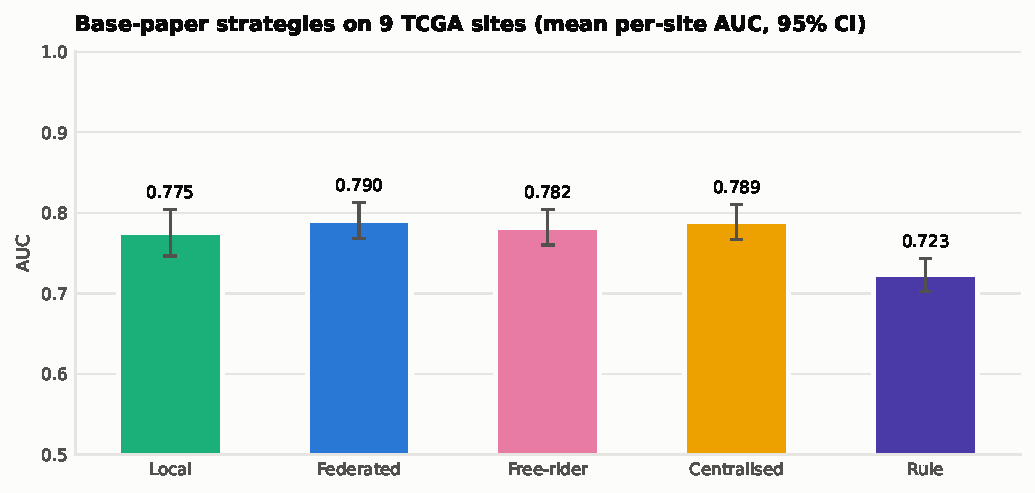
\includegraphics[width=\columnwidth]{figures/figure12_base_paper.pdf}
\caption{Base-paper strategies on the TCGA sites: mean per-site test AUC with 95\% CI over 20 seeds.}
\label{fig:base_paper}
\end{figure}

\begin{figure}[!ht]
\centering
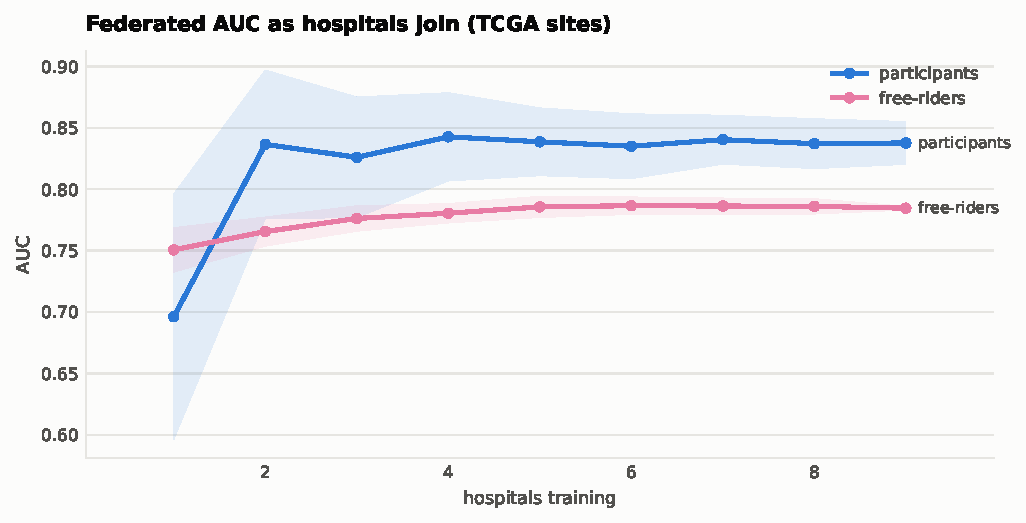
\includegraphics[width=\columnwidth]{figures/figure13_learning_curve.pdf}
\caption{FedAvg AUC for participating sites and for free-riders (non-participating sites and the external small-site pool) as sites join in random order.}
\label{fig:learning_curve}
\end{figure}

\subsection{Centralised Baselines and Feature Sets}
Table~\ref{tab:centralized} compares feature sets with repeated cross-validation. The full clinical set reaches \cvFull{} with the NumPy model used in federation. Adding the protein principal components \emph{lowers} discrimination (paired difference $\cvProtDiff$), and protein features alone reach only \cvProt{}: with roughly 115 components for \nTrain{} training patients the linear model over-fits. Removing the post-surgical pathology features costs $\cvPreopDiff$ (pre-operative model \cvPreop{}). The remaining experiments therefore use the full clinical feature set; the multimodal and pre-operative variants are reported in the ablation.

\begin{table*}[t]
\caption{Centralised baselines: mean AUC over repeated stratified cross-validation (25 folds, 5$\times$5) on the 347-patient cohort. All preprocessing is fitted inside each training fold.}
\centering\small
\begin{tabular}{lccccc}
\toprule
Model & Clinical (full) & Clinical (pre-op) & Protein only & Full + protein & Pre-op + protein \\
\midrule
NumPy LR (ours) & 0.818 & 0.642 & 0.574 & 0.659 & 0.595 \\
LR (L2) & 0.824 & 0.661 & 0.633 & 0.682 & 0.638 \\
LR (L1) & 0.831 & 0.662 & 0.637 & 0.712 & 0.659 \\
Random forest & 0.803 & 0.644 & 0.599 & 0.782 & 0.627 \\
MLP & 0.792 & 0.670 & 0.599 & 0.664 & 0.623 \\
\bottomrule
\end{tabular}
\label{tab:centralized}
\end{table*}


\subsection{Client Drift under Statistical Heterogeneity (H1)}
Table~\ref{tab:drift} and Fig.~\ref{fig:drift} report client drift (Eq.~\ref{eq:drift}). Drift grows with heterogeneity (FedAvg: \driftAvgIID{} at $\alpha=100$ to \driftAvgSkew{} at $\alpha=0.1$), and FedProx reduces it by \driftRedMin--\driftRedMax\% at every $\alpha$, with 95\% CIs far from zero; increasing $\mu$ from 0 to 1 lowers drift monotonically (\driftMuZero{} to \driftMuOne{} at $\alpha=0.5$). H1 is supported. The reduction in drift does not translate into higher test AUC without DP: no paired AUC difference is significant, because the convex logistic objective lets FedAvg reach a good solution regardless.

\begin{table*}[t]
\caption{Client drift $\bar d = \mathrm{mean}_{t,k}\|w_k^t - w^{t-1}\|_2$ without DP (3 clients, 20 seeds, mean $\pm$ sd). Spread = max$-$min T3/T4 rate across clients. Last column: paired FedProx$-$FedAvg test-AUC difference with 95\% CI.}
\centering\small
\begin{tabular}{cccccc}
\toprule
$\alpha$ & Spread & FedAvg drift & FedProx drift & Reduction \% [95\% CI] & $\Delta$AUC [95\% CI] \\
\midrule
100 & 0.07 & $0.206 \pm 0.023$ & $0.140 \pm 0.013$ & $32.0$ [31.4, 32.5] & $+0.0022\ [\ensuremath{-}0.0012, +0.0057]$ \\
10 & 0.20 & $0.263 \pm 0.053$ & $0.175 \pm 0.033$ & $33.2$ [32.6, 33.8] & $+0.0018\ [\ensuremath{-}0.0013, +0.0049]$ \\
1 & 0.55 & $0.525 \pm 0.157$ & $0.337 \pm 0.096$ & $35.6$ [34.9, 36.2] & $+0.0019\ [\ensuremath{-}0.0009, +0.0046]$ \\
0.5 & 0.68 & $0.599 \pm 0.165$ & $0.382 \pm 0.100$ & $36.0$ [35.5, 36.5] & $+0.0016\ [\ensuremath{-}0.0024, +0.0056]$ \\
0.1 & 0.84 & $0.770 \pm 0.181$ & $0.488 \pm 0.110$ & $36.4$ [35.9, 36.9] & $+0.0018\ [\ensuremath{-}0.0009, +0.0044]$ \\
\bottomrule
\end{tabular}
\label{tab:drift}
\end{table*}


\begin{figure}[!ht]
\centering
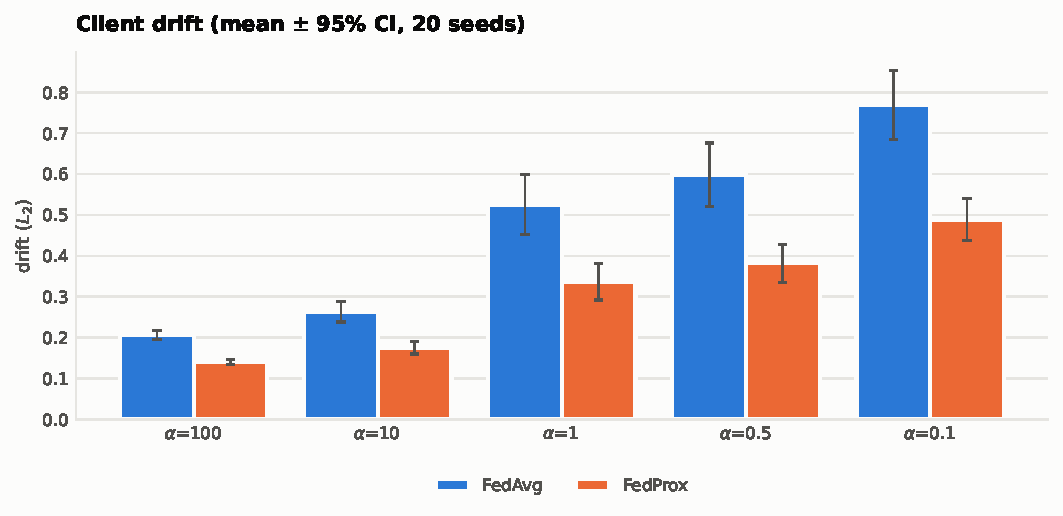
\includegraphics[width=\columnwidth]{figures/figure5_drift.pdf}
\caption{Client drift (Eq.~\ref{eq:drift}) of FedAvg and FedProx across Dirichlet $\alpha$ (mean and 95\% CI over 20 seeds).}
\label{fig:drift}
\end{figure}

\subsection{Privacy--Utility Trade-off (H2)}
Fig.~\ref{fig:privacy_utility} shows global test AUC against the privacy budget at $\alpha=10$. Without DP FedAvg reaches \auNoDP{}. Weak privacy is almost free ($\varepsilon=10$: \auAvgTen{}, paired loss $\auLossTen$), whereas strong privacy is costly ($\varepsilon=2$: $\auLossTwo$; $\varepsilon=1$: $\auLossOne$; $\varepsilon=0.5$: $\auLossHalf$). With 20 paired seeds the degradation at $\varepsilon \le 2$ is significant, supporting H2.

\begin{figure}[!ht]
\centering
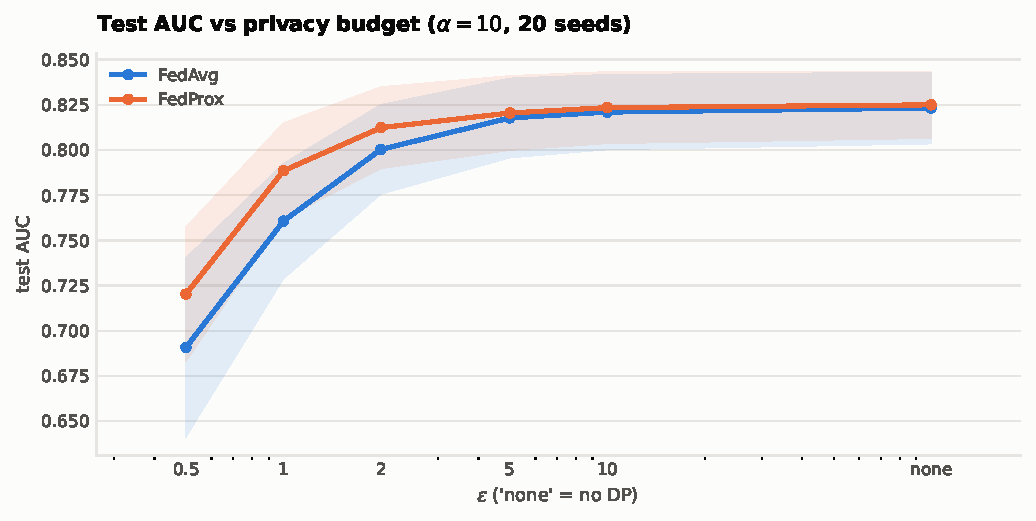
\includegraphics[width=\columnwidth]{figures/figure3_privacy_utility.pdf}
\caption{Global test AUC versus privacy budget $\varepsilon$ ($\alpha=10$, $K=3$; mean and 95\% CI over 20 seeds).}
\label{fig:privacy_utility}
\end{figure}

\subsection{FedProx under Joint Privacy and Heterogeneity (H3)}
Table~\ref{tab:interaction} and Fig.~\ref{fig:heatmap} cross label skew with privacy. Without DP, FedProx and FedAvg are indistinguishable (largest mean difference \gridNoDPmax). Under DP, FedProx is significantly better in \gridSup{} of \gridCells{} cells, by \gridOneHalfMin--\gridOneHalfMax{} AUC at $\varepsilon \in \{1, 0.5\}$, largely independent of $\alpha$. A step-size control explains this: a FedAvg run with half the learning rate matches FedProx (FedProx better in only \gridSupCtl{} of \gridCells{} cells; largest mean difference \gridCtlOneHalfMax{} at $\varepsilon \le 1$). Under DP the proximal term acts mainly as a smaller effective step that damps the injected noise, rather than as a correction for heterogeneity. H3 is therefore supported only in this qualified sense.

\begin{table*}[t]
\caption{Global test AUC under joint label skew ($\alpha$) and privacy ($\varepsilon$), 3 clients, mean over 20 seeds. FedAvg ($\eta/2$) is a step-size control. $\Delta$ = paired FedProx$-$FedAvg difference; bold = 95\% CI excludes 0.}
\centering\small
\begin{tabular}{llcccccc}
\toprule
 & Model & no DP & $\varepsilon=10$ & $\varepsilon=5$ & $\varepsilon=2$ & $\varepsilon=1$ & $\varepsilon=0.5$ \\
\midrule
$\alpha=10$ & FedAvg & 0.823 & 0.821 & 0.818 & 0.800 & 0.761 & 0.691 \\
 & FedProx & 0.825 & 0.823 & 0.821 & 0.812 & 0.789 & 0.720 \\
 & FedAvg ($\eta/2$) & 0.826 & 0.821 & 0.820 & 0.812 & 0.786 & 0.718 \\
 & $\Delta$ Prox$-$Avg & -- & +0.002 & +0.003 & \textbf{+0.012} & \textbf{+0.028} & \textbf{+0.029} \\
\midrule
$\alpha=1$ & FedAvg & 0.823 & 0.821 & 0.818 & 0.801 & 0.757 & 0.688 \\
 & FedProx & 0.825 & 0.823 & 0.820 & 0.812 & 0.787 & 0.717 \\
 & FedAvg ($\eta/2$) & 0.825 & 0.821 & 0.820 & 0.812 & 0.786 & 0.715 \\
 & $\Delta$ Prox$-$Avg & -- & +0.002 & +0.002 & \textbf{+0.012} & \textbf{+0.030} & \textbf{+0.029} \\
\midrule
$\alpha=0.5$ & FedAvg & 0.824 & 0.821 & 0.818 & 0.799 & 0.758 & 0.687 \\
 & FedProx & 0.826 & 0.823 & 0.820 & 0.811 & 0.787 & 0.715 \\
 & FedAvg ($\eta/2$) & 0.826 & 0.821 & 0.820 & 0.811 & 0.784 & 0.715 \\
 & $\Delta$ Prox$-$Avg & -- & +0.002 & +0.002 & \textbf{+0.012} & \textbf{+0.029} & \textbf{+0.028} \\
\midrule
$\alpha=0.1$ & FedAvg & 0.825 & 0.821 & 0.818 & 0.796 & 0.753 & 0.684 \\
 & FedProx & 0.826 & 0.823 & 0.820 & 0.809 & 0.782 & 0.713 \\
 & FedAvg ($\eta/2$) & 0.827 & 0.821 & 0.820 & 0.810 & 0.782 & 0.712 \\
 & $\Delta$ Prox$-$Avg & -- & +0.002 & +0.002 & \textbf{+0.012} & \textbf{+0.029} & \textbf{+0.029} \\
\bottomrule
\end{tabular}
\label{tab:interaction}
\end{table*}


\begin{figure}[!ht]
\centering
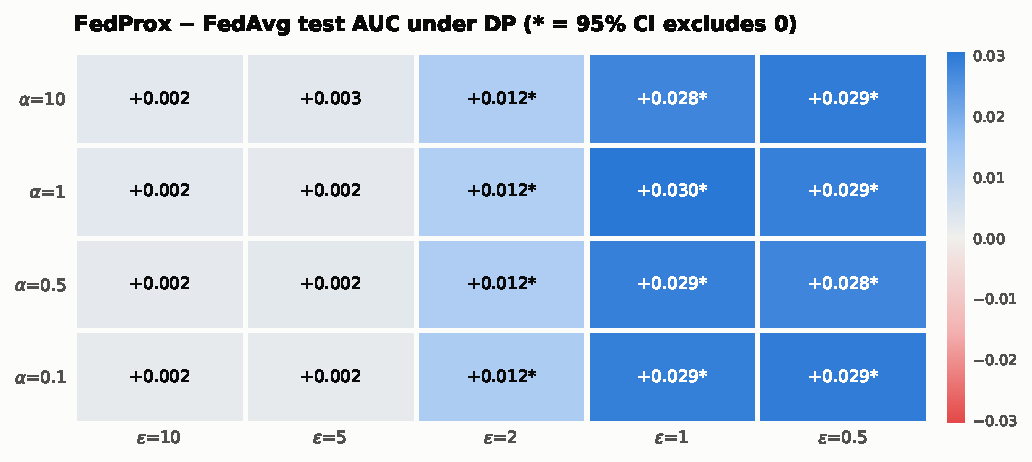
\includegraphics[width=\columnwidth]{figures/figure4_heatmap.pdf}
\caption{Paired FedProx$-$FedAvg test-AUC difference across $\alpha$ and $\varepsilon$ (20 seeds; * = 95\% CI excludes 0).}
\label{fig:heatmap}
\end{figure}

\subsection{Personalised Adaptation (H4)}
Table~\ref{tab:local_adaptation} and Fig.~\ref{fig:pfl} evaluate each client on its own test split ($\alpha=0.5$). With three clients, FedProx reaches \pflProxThree{} per client against \pflLocalThree{} for local-only models, and personalised fine-tuning (PFL) reaches \pflPFLThree{} (PFL$-$Local $=\pflGainThree$). PFL does not improve on the global FedProx model (PFL$-$FedProx $=\pflVsProxThree$ for $K=3$, $\pflVsProxTen$ for $K=10$). With $K=10$ the comparison is again in favour of collaboration (PFL$-$Local $=\pflGainTen$). Because many clients have a single-class test split under strong skew, these averages cover only the clients with a defined AUC (Table~\ref{tab:local_adaptation}). H4 is supported for PFL versus local training, but not for PFL versus the global model.

\begin{table*}[t]
\caption{Mean per-client test AUC ($\alpha=0.5$, 20 seeds) over clients whose local test split contains both classes (\#def. = mean number of such clients). PFL = proximal fine-tuning of the FedProx model. Paired differences with 95\% CI.}
\centering\small
\begin{tabular}{ccccccrr}
\toprule
$K$ & \#def. & Local & FedAvg & FedProx & PFL & PFL$-$Local & PFL$-$FedProx \\
\midrule
3 & 2.2 & 0.754 & 0.810 & 0.811 & 0.805 & $+0.051\ [+0.015, +0.086]$ & $-0.006\ [\ensuremath{-}0.022, +0.011]$ \\
5 & 2.9 & 0.796 & 0.820 & 0.817 & 0.814 & $+0.018\ [\ensuremath{-}0.021, +0.057]$ & $-0.003\ [\ensuremath{-}0.011, +0.005]$ \\
10 & 3.5 & 0.785 & 0.840 & 0.841 & 0.838 & $+0.053\ [+0.010, +0.096]$ & $-0.003\ [\ensuremath{-}0.014, +0.007]$ \\
\bottomrule
\end{tabular}
\label{tab:local_adaptation}
\end{table*}


\begin{figure}[!ht]
\centering
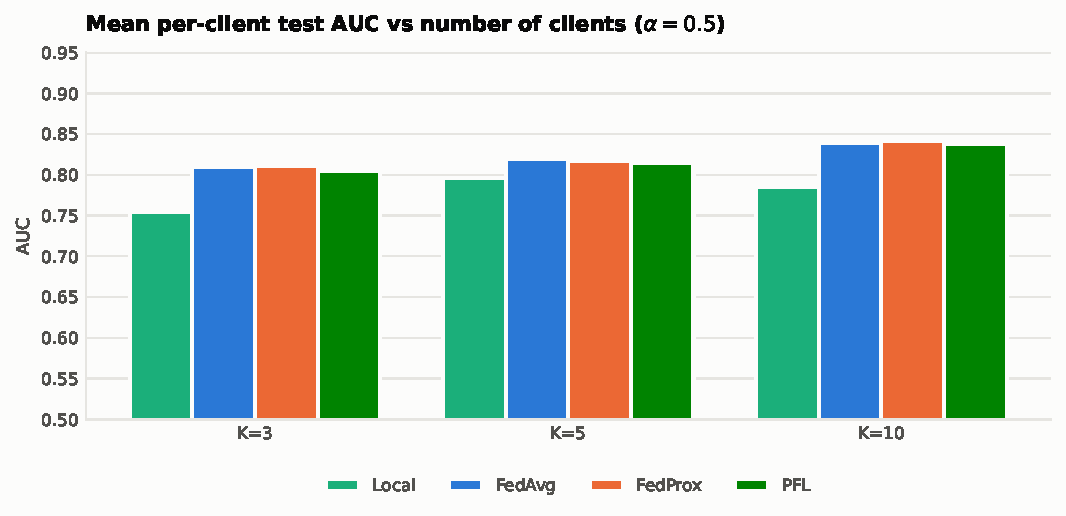
\includegraphics[width=\columnwidth]{figures/figure10_fedprox_scaling_benefit.pdf}
\caption{Mean per-client test AUC of local, FedAvg, FedProx and personalised models for $K \in \{3, 5, 10\}$ clients ($\alpha=0.5$, 20 seeds).}
\label{fig:pfl}
\end{figure}

\subsection{Contribution Valuation under Privacy Noise (H5)}
\label{sec:contribution_valuation}
Without DP, exact Shapley values are positive for every client and track client size only moderately (Spearman with size: \shSizeThree{} for $K=3$, \shSizeTen{} for $K=10$); LOO rankings agree with Shapley rankings only partially (\shLooThree{} for $K=3$, \shLooTen{} for $K=10$), because LOO ignores sub-coalitions and becomes nearly zero when one client is redundant.

Table~\ref{tab:wilcoxon_results} and Figs.~\ref{fig:shapley_instability}--\ref{fig:shapley_scaling_instability} quantify how DP changes these values. Each DP realisation is compared with the no-DP ranking of the same partition, so the Shapley computation itself contributes no randomness (exact enumeration). Rank agreement falls monotonically as privacy strengthens: for $K=3$, Spearman $\rho$ drops from \shRhoTenThree{} at $\varepsilon=10$ to \shRhoHalfThree{} at $\varepsilon=0.5$, and for $K=10$ from \shRhoTenTen{} to \shRhoHalfTen{}. Even the weakest budget leaves $\rho$ well below 0.90 (one-sided Wilcoxon $p<0.01$ in every configuration). The probability that the no-DP top contributor is still ranked first falls from \shTSTenThree{} to \shTSHalfThree{} for $K=3$ (chance 0.33) and from \shTSTenTen{} to \shTSHalfTen{} for $K=10$ (chance 0.10), and at $\varepsilon=0.5$ the rank-reversal rate reaches \shRRHalfTen{} for $K=10$. The overall rank correlation degrades by a similar amount for every federation size, whereas exact ranks and the top contributor are least stable in larger federations. H5 is supported: an incentive scheme that pays hospitals according to Shapley values computed from DP-trained models would frequently reward the wrong hospital.

\begin{table*}[t]
\caption{Stability of exact Shapley rankings under DP relative to the no-DP ranking (20 partitions; 5, 5, 2 noise realisations per partition for $K=3, 5, 10$). TS = probability that the no-DP top contributor is still ranked first (chance = $1/K$). $p$: one-sided Wilcoxon test of $\rho-0.90<0$.}
\centering\small
\begin{tabular}{ccccccc}
\toprule
$K$ & $\varepsilon$ & Spearman $\rho$ [95\% CI] & Rank reversal & TS & Chance TS & $p$ \\
\midrule
3 & 10 & 0.68 [0.50, 0.85] & 0.30 & 0.79 & 0.33 & 0.007 \\
3 & 5 & 0.54 [0.35, 0.73] & 0.38 & 0.73 & 0.33 & 4.1e-4 \\
3 & 2 & 0.40 [0.21, 0.60] & 0.48 & 0.61 & 0.33 & 1.4e-4 \\
3 & 1 & 0.36 [0.16, 0.56] & 0.51 & 0.56 & 0.33 & 6.4e-5 \\
3 & 0.5 & 0.25 [0.07, 0.43] & 0.57 & 0.51 & 0.33 & 4.3e-5 \\
\midrule
5 & 10 & 0.66 [0.55, 0.78] & 0.52 & 0.65 & 0.20 & 7.0e-5 \\
5 & 5 & 0.59 [0.45, 0.72] & 0.59 & 0.60 & 0.20 & 5.1e-5 \\
5 & 2 & 0.46 [0.30, 0.62] & 0.66 & 0.48 & 0.20 & 4.4e-5 \\
5 & 1 & 0.37 [0.21, 0.52] & 0.73 & 0.40 & 0.20 & 4.4e-5 \\
5 & 0.5 & 0.30 [0.15, 0.45] & 0.74 & 0.41 & 0.20 & 4.4e-5 \\
\midrule
10 & 10 & 0.73 [0.67, 0.79] & 0.76 & 0.62 & 0.10 & 5.2e-5 \\
10 & 5 & 0.66 [0.58, 0.75] & 0.77 & 0.60 & 0.10 & 9.5e-7 \\
10 & 2 & 0.55 [0.45, 0.64] & 0.79 & 0.45 & 0.10 & 4.4e-5 \\
10 & 1 & 0.48 [0.39, 0.56] & 0.82 & 0.38 & 0.10 & 4.4e-5 \\
10 & 0.5 & 0.36 [0.26, 0.47] & 0.88 & 0.30 & 0.10 & 4.4e-5 \\
\bottomrule
\end{tabular}
\label{tab:wilcoxon_results}
\end{table*}


\begin{figure}[!ht]
\centering
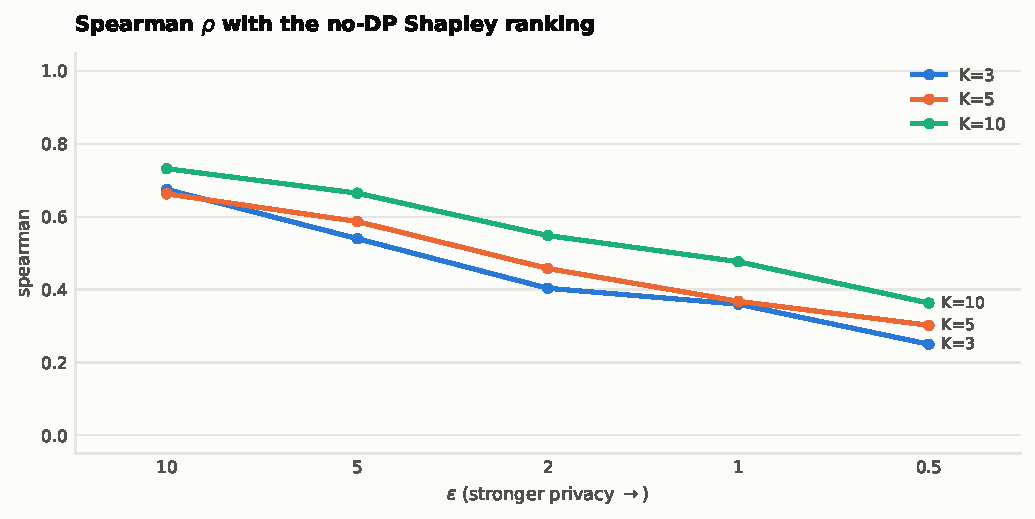
\includegraphics[width=\columnwidth]{figures/figure9_shapley_instability.pdf}
\caption{Spearman correlation between DP and no-DP exact Shapley rankings versus $\varepsilon$ for $K \in \{3, 5, 10\}$ clients (20 partitions).}
\label{fig:shapley_instability}
\end{figure}

\begin{figure}[!ht]
\centering
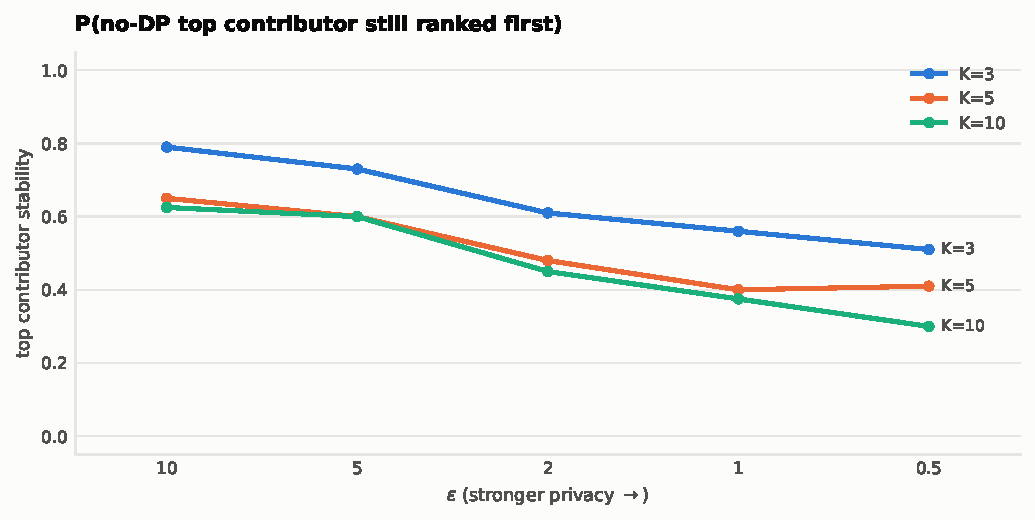
\includegraphics[width=\columnwidth]{figures/figure11_shapley_scaling_instability.pdf}
\caption{Top-contributor stability (probability that the no-DP top contributor stays first under DP) versus $\varepsilon$; chance level is $1/K$.}
\label{fig:shapley_scaling_instability}
\end{figure}

\begin{figure}[!ht]
\centering
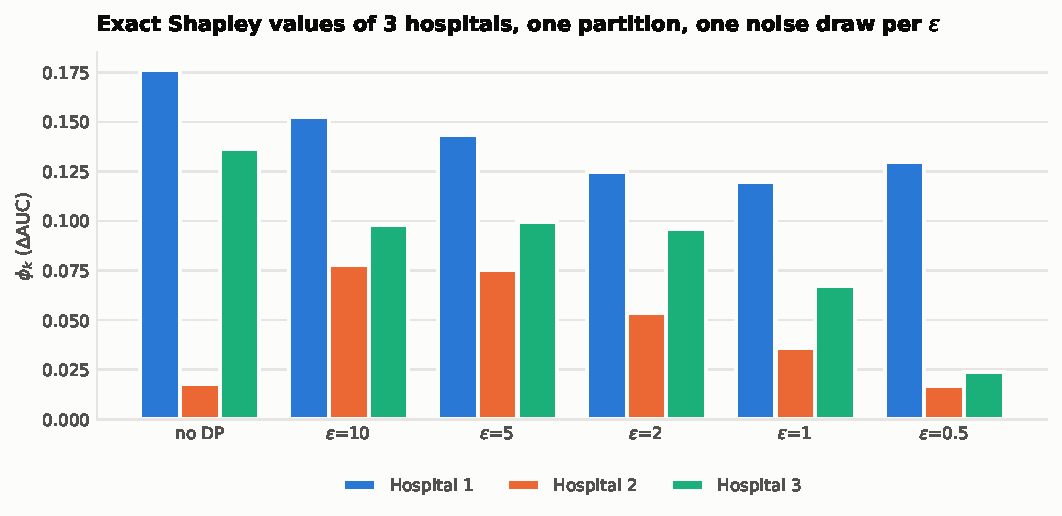
\includegraphics[width=\columnwidth]{figures/figure6_shapley.pdf}
\caption{Exact Shapley values of three clients for one partition: no DP and one DP noise draw per $\varepsilon$.}
\label{fig:shapley_volatility}
\end{figure}

\subsection{Empirical Membership-Inference Evaluation (H7)}
Without DP the confidence-threshold attack is at chance level (attack AUC $\miaNoDP$), and it stays there under DP ($\varepsilon=1$: $\miaOne$; $\varepsilon=0.5$: $\miaHalf$). The positive control confirms that the attack works when a model memorises its training data (AUC $\miaCtl$). The 18-feature logistic model generalises well (train$-$test AUC gap $\miaGap$), so there is little membership signal for DP to remove. The formal DP guarantee still holds, but its \emph{empirical} benefit cannot be demonstrated with this attack, and H7 is not supported. (The previously reported reduction from 0.568 to 0.480 arose in a pipeline whose identifier features let the model memorise individual patients.)

\begin{figure}[!ht]
\centering
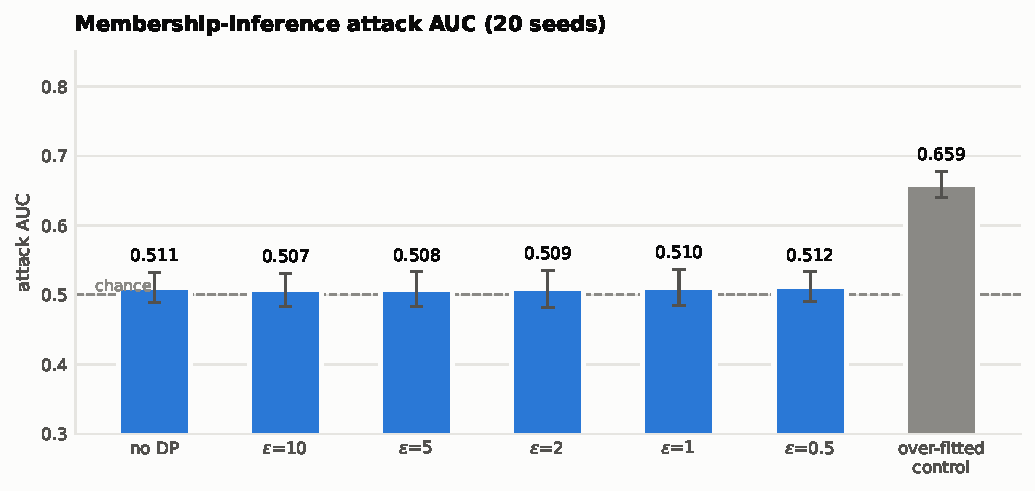
\includegraphics[width=\columnwidth]{figures/figure7_mia.pdf}
\caption{Membership-inference attack AUC (mean and 95\% CI over 20 seeds) without DP, under DP, and for an over-fitted positive control. 0.5 = chance.}
\label{fig:mia}
\end{figure}

\subsection{Controlled Distribution-Shift Stress Test (H6)}
Under synthetic covariate shift the FedProx model degrades gracefully (AUC \shiftBase{} $\to$ \shiftCovTwo{} at severity 2), while concept shift, which flips labels, drives it to \shiftConTwo{} (Fig.~\ref{fig:stress_test}). This is a sensitivity analysis on perturbed copies of the test split, not an external validation.

\begin{figure}[!ht]
\centering
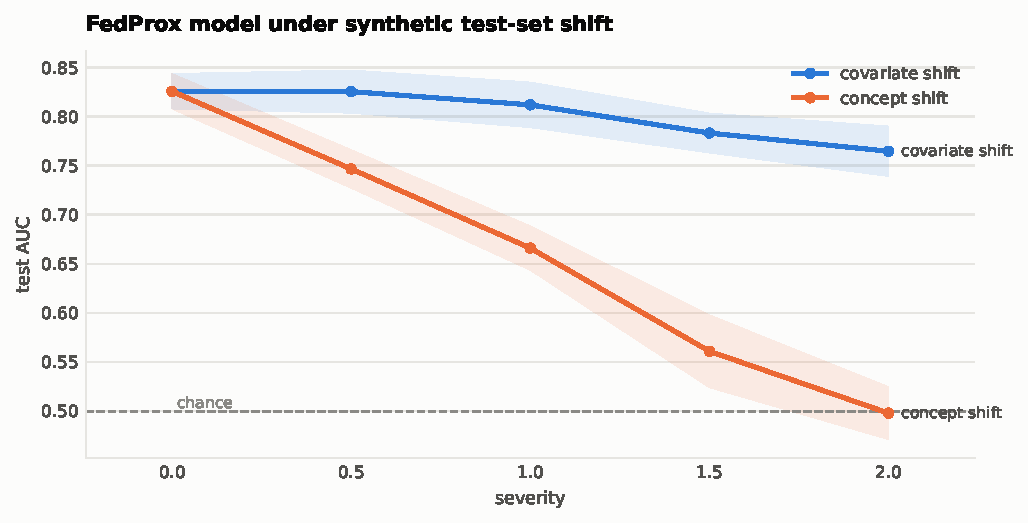
\includegraphics[width=\columnwidth]{figures/figure8_stress_test.pdf}
\caption{FedProx test AUC under synthetic covariate and concept shift of the test split (20 seeds).}
\label{fig:stress_test}
\end{figure}

\subsection{Ablation}
Table~\ref{tab:global_ablation} summarises the components on the global test split ($K=3$, $\alpha=0.5$). FedAvg (\abAvg{}) and FedProx (\abProx{}) match centralised training (\abCen{}). DP costs little at $\varepsilon=5$ (\abDPFive{}) and more at $\varepsilon=1$ (\abDPOne{}). Using only pre-operative features (\abPreop{}) or adding protein components (\abProt{}) both reduce discrimination substantially.

\begin{table}[t]
\caption{Ablation on the global test split ($K=3$, $\alpha=0.5$, 20 seeds, mean $\pm$ sd; paired difference to FedProx with 95\% CI).}
\centering\scriptsize
\setlength{\tabcolsep}{4pt}
\begin{tabular}{p{2.9cm}cc}
\toprule
Configuration & Test AUC & vs FedProx \\
\midrule
Centralised (pooled data) & $0.823 \pm 0.042$ & $-0.003\ [\ensuremath{-}0.008, +0.002]$ \\
FedAvg & $0.824 \pm 0.041$ & $-0.002\ [\ensuremath{-}0.006, +0.002]$ \\
FedProx & $0.826 \pm 0.038$ & reference \\
FedProx + DP ($\varepsilon$=5) & $0.820 \pm 0.045$ & $-0.006\ [\ensuremath{-}0.012, +0.001]$ \\
FedProx + DP ($\varepsilon$=1) & $0.787 \pm 0.058$ & $-0.039\ [\ensuremath{-}0.056, \ensuremath{-}0.022]$ \\
FedProx: pre-op features only & $0.659 \pm 0.062$ & $-0.167\ [\ensuremath{-}0.193, \ensuremath{-}0.141]$ \\
FedProx: clinical (full) + protein PCs & $0.682 \pm 0.050$ & $-0.144\ [\ensuremath{-}0.166, \ensuremath{-}0.122]$ \\
\bottomrule
\end{tabular}
\label{tab:global_ablation}
\end{table}


\section{Survival Analysis Limitation}
A federated Cox model was implemented, but the matched cohort contains only \nEvents{} deaths among \nMatched{} patients (\nEventsTest{} in the reference test split), so out-of-sample survival discrimination cannot be estimated reliably. No survival claims are made.

\section{Discussion}
The 19-hospital evaluation changes the weight of the evidence in three ways. First, the base paper's sustainability argument is now confirmed on its own data and under a different training protocol, and extended to leave-one-country-out external validation. Second, the cost of DP depends mainly on cohort size: it is almost free with \pNineN{} patients and substantial with 347. Third, DP's main clinical side effect at scale is not lost discrimination but over-confident predictions, which a cheap local recalibration fixes. That is a concrete deployment recipe: train with DP in the federation, then let each new hospital recalibrate on a small local sample. The instability of Shapley rankings under DP also holds on real hospitals: it is milder than on TCGA at weak privacy, but appears at strong privacy where accuracy is unchanged, and the top contributor is fragile at every privacy level. Contribution-based payments in private federations therefore need noise-robust valuation regardless of how cheap privacy is for accuracy. OSA-Shapley provides one: it accounts for privacy honestly, re-uses common noise across coalitions and, at the same budget, recovers rankings that retraining loses. Its limitation is the one-shot approximation of the federated model, which is accurate for convex models trained to convergence but untested for deep networks.

On TCGA-PRAD, four results stand out. First, replicating the base paper on real TCGA sites reproduces its sustainability argument: joining a federation brings a hospital no significant local gain over its own model, yet a federated model serves non-participating hospitals almost as well as participants, and most of the free-rider benefit is reached with four to five contributing sites. Second, privacy has a clear utility price below $\varepsilon \approx 2$, and FedProx softens it, but a step-size control shows that the benefit comes from damping noisy local steps rather than from correcting heterogeneity; without DP, FedProx reduces client drift by about a third without changing accuracy. Third, DP noise severely destabilises Shapley-based contribution rankings at every federation size, which matters for any payment or reputation scheme built on valuations of privately trained models. Fourth, the empirical privacy audit is uninformative for this low-capacity model: membership inference is at chance even without DP.

The corrected pipeline also changes two substantive conclusions of earlier drafts. Proteomic principal components do not improve staging on this cohort; they reduce AUC. And much of the predictive signal comes from post-surgical pathology variables that are recorded together with the pathologic T label, so the clinically realistic pre-operative task is considerably harder (AUC \cvPreop{}).

\subsection{Threats to Validity}
\label{sec:threats_validity}

\subsubsection{Internal Validity}
Hyper-parameters introduced in the revision (OSA-Shapley local steps, FedAdam server learning rate, federated MLP learning rate, learning rates for subsampled DP) were tuned on four splits and evaluated on twenty disjoint ones. PCa-19 hospitals are real, but its data were harmonised by the base paper's authors from published supplementary files, and records with missing values were discarded by them. Two PCa-19 hospitals have fewer than 50 patients, so their per-hospital AUCs are noisy; we therefore report both hospital-averaged and patient-weighted summaries. On TCGA, Dirichlet clients are simulated; the real-site analysis uses TCGA tissue-source sites, which are biobanks rather than independent clinical deployments, and their test splits are small (5--19 patients), so single-site AUCs are noisy and only averages over seeds should be interpreted. Hyper-parameters were selected by cross-validation on the same cohort. Exact Shapley values were computed for up to 10 clients; larger federations would require approximation.

\subsubsection{External Validity}
Both evaluations are retrospective. PCa-19 covers eight countries with pre-biopsy variables, and its leave-one-country-out results are the strongest evidence of transportability in this study; prospective validation is still required before clinical use. On TCGA-PRAD the strongest predictors (Gleason pattern, pathologic N) are post-surgical, and PSA is unavailable, so TCGA results concern methodology rather than a deployable tool.

\subsubsection{Privacy Validity}
The guarantee is per patient for the analysed cohort (one sample per patient) and treats client sizes and the shared preprocessing statistics as public. The main experiments use full-batch updates ($q=1$) with conservative accounting; Poisson subsampling with sampled-Gaussian accounting gives a tighter bound but no utility gain. OSA-Shapley's guarantee covers the valuation release; if the training run is also released, the two budgets compose. The empirical audit uses one confidence-threshold attack and does not cover gradient-reconstruction or model-inversion attacks.

\subsubsection{Statistical Validity}
All comparisons are paired over 20 seeds; seed-level replicates share the same patients, so the CIs describe variability across splits and partitions rather than across independent cohorts. For leave-one-country-out results we therefore treat the eight countries as the independent units ($n=8$). Cross-validation fold differences are correlated, so their CIs are indicative.

\subsection{Reproducibility Statement}
All results, tables and figures are regenerated from code: \texttt{python run\_all.py} and \texttt{python run\_pca19.py} recompute every experiment into \texttt{results/final/}, \texttt{python -m fl\_study.validate} runs 34 automated checks (cohort counts, the sampled-Gaussian accountant against numerical integration and a published value, subsampled DP-SGD, OSA-Shapley against exact retraining, the SCAFFOLD and FedAdam implementations, agreement of our re-implementation with the base paper's own code on PCa-19, leave-one-country-out preprocessing isolation, stratified-vs-exact Shapley agreement, calibration and recalibration formulas, absence of identifier features, train-only preprocessing, RDP accountant against the closed form, empirical noise scale, clipping bound, Shapley axioms, equivalence of vectorised and per-coalition training, and reproducibility), and \texttt{python Paper/generate\_paper\_assets.py} writes every number in this manuscript. Code: \url{https://github.com/JeyanthPonnaluri/Mini_Project_RVR}.

\section{Future Work}
Future work will extend OSA-Shapley to non-convex models (where one-shot averaging is a poorer proxy), combine it with secure aggregation, study privacy-preserving federated recalibration, validate the PCa-19 model prospectively, and use cohorts with enough survival events.

\section{Conclusion}
We studied privacy, heterogeneity, personalisation and contribution valuation in federated prostate-cancer risk prediction with one leakage-free pipeline, on the base paper's own 19 real hospitals and on TCGA-PRAD. On the base paper's data, we reproduce its published protocol exactly and confirm its sustainability argument under ours: federated models match pooled training, joining brings no significant average local gain, and free-riders are served almost as well. Leave-one-country-out validation shows that discrimination transports but calibration does not. DP is nearly free in AUC at this scale but makes predictions over-confident, and local recalibration on a small sample repairs both problems. On both cohorts, FedProx's advantage under DP equals that of a smaller learning rate, and DP noise destabilises Shapley contribution rankings, even on real hospitals where it does not change accuracy. Retraining-based valuation under DP spends the privacy budget hundreds of times over and, at an honest budget, loses the ranking. OSA-Shapley, which post-processes one DP-trained model per hospital, recovers it at a single budget and makes exact valuation of all 19 hospitals tractable. Stronger optimisers, non-linear models and subsampled DP accounting did not change these conclusions.

\bibliographystyle{IEEEtran}
\bibliography{references}

\end{document}
